\documentclass[a4paper,11pt]{article}
\usepackage[margin=2.5cm,left=1.5cm,right=1.5cm]{geometry}
\usepackage{graphicx}
\usepackage{hyperref}
\usepackage{booktabs}
\usepackage{longtable}
\usepackage{parskip}
\usepackage{titlesec}
\usepackage{fancyhdr}
\usepackage{float}
\usepackage{pdflscape}
\usepackage{multicol}
\usepackage[export]{adjustbox}
\setlength{\headheight}{13.6pt}

\newcommand{\sectionbreak}{\clearpage}

% Allow line breaks after underscores globally
\let\oldunderscore\_
\renewcommand{\_}{\oldunderscore\allowbreak}

% Formula graphic on its own landscape page
\newcommand{\formulagraph}[4][]{%
\vspace*{\fill}
\begin{figure}[H]
\centering
\includegraphics[max width=\linewidth, max height=0.8\textheight, keepaspectratio, #1]{#2}
\caption{#3}
\label{#4}
\end{figure}
\vspace*{\fill}\null
}

\hypersetup{
	colorlinks=true,
	linkcolor=blue,
	urlcolor=blue,
	pdftitle={Lotus T4e ECU},
	pdfauthor={J.F.},
	pdfsubject={Engine Management \& Tuning Guide},
}

\pagestyle{fancy}
\fancyhf{}
\fancyhead[L]{Lotus T4e ECU - Engine Management \& Tuning Guide}
\fancyhead[R]{\leftmark}
\fancyfoot[C]{\thepage}

\title{Lotus T4e ECU\\[0.5em]\large Engine Management \& Tuning Guide\\[0.5em]\normalsize Elise / Exige / 211 (Toyota 1ZZ-FE / 2ZZ-GE)\\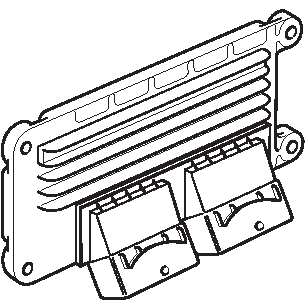
\includegraphics[width=0.6\linewidth]{t4e.pdf}}
\author{Reverse Engineered by J.F.}
\date{\today}

\begin{document}
\maketitle
\section{Table of contents}
\tableofcontents
\newpage
\section{List of figures}
\listoffigures
\newpage
\section{List of tables}
\listoftables
\newpage

% =============================================================================
\section{Introduction}
% =============================================================================

This document describes the internal workings of the Lotus T4e ECU (MPC563-based)
used in Lotus Elise, Exige, and 211 models equipped with the Toyota 1ZZ-FE and
2ZZ-GE engines. It is intended as both a technical reference and a tuning guide.

The ECU firmware has been reverse engineered from the binary, and the formulas
presented here are derived directly from the decompiled code.

\subsection{Audience}

This guide is meant for Lotus owners who want full control over their car.
It represents more than a hundred hours of reverse engineering work, shared
freely because I believe every owner should be able to understand and tweak
their own ECU.

However, I am not willing for professional tuners to use this work to develop
tunes sold to customers without supporting the project, either financially or by
contributing improvements. This is why the entire project, including this
document, is released under the
\textbf{Creative Commons Attribution-NonCommercial-ShareAlike (CC BY-NC-SA)}
license. Any material and knowledge contained here cannot be used commercially
(i.e. by professionals requesting money to tune cars) unless an agreement has
been reached with the project author.

Professional tuners are welcome to use this material as long as they do so
without commercial intent, meaning the resulting tune must be made freely
available under the same \textbf{CC BY-NC-SA} license. Charging separately
for hardware, installation, or other services unrelated to the tune itself
remains perfectly acceptable.

\textbf{If you are a professional without intent to support this project or
publish your work freely, STOP READING HERE.}

\subsection{Workflow}

This guide is the end product of a multi-step reverse engineering pipeline:

\begin{enumerate}
	\item \textbf{Original firmware} --- the binary is read from the ECU flash.
	\item \textbf{Ghidra} --- the binary is disassembled and decompiled into
	      readable C code. Functions, variables, and data structures are
	      identified and renamed.
	\item \textbf{Identifying calibration data} --- maps and parameters are
	      tagged as \texttt{CAL\_} (calibration) or \texttt{LEA\_} (learned
	      adaptive values).
	\item \textbf{Export script} --- a Ghidra script exports the identified
	      symbols into RomRaider definition files.
	\item \textbf{RomRaider} --- the definition files allow editing the
	      calibration maps in \texttt{calrom.bin}.
	\item \textbf{Exported C code} --- Ghidra's decompiled C output is
	      exported for further analysis.
	\item \textbf{Claude AI assistant} --- the exported C code is analyzed
	      with Claude to trace formulas, identify logic, and produce the
	      descriptions and diagrams in this guide.
	\item \textbf{Human review} --- all AI-generated text and diagrams are
	      thoroughly reviewed before publication.
\end{enumerate}

Every symbol identified in the source code as \texttt{CAL\_} or \texttt{LEA\_}
is automatically exported into a RomRaider definition. The prefix is removed,
the first word becomes the category, and all underscores are replaced by
spaces. For example, \texttt{CAL\_ign\_adv\_low\_cam\_base} appears in
RomRaider under the category \emph{ign} as \emph{adv low cam base}. The same
naming convention is used in the formula diagrams throughout this guide.

% =============================================================================
\section{RomRaider Definition}
% =============================================================================

\subsection{Compatibility}

The \texttt{T4E090\_def.xml} is a comprehensive definition that covers all
\texttt{CAL\_} parameters discussed in this guide, allowing them to be edited
in RomRaider. It also enables visualisation of \texttt{LEA\_} parameters;
these can be edited too, but modifying learned adaptation values has little
effect since the ECU will overwrite them sooner or later.

The following calibrations use the exact same software:

\begin{multicols}{4}
\begin{itemize}
	\item A131E0018
	\item A121E0013
	\item A128E0032
	\item A129E0001
	\item B121E0014
	\item A128E0036
	\item A127E0062
	\item A127E0064
	\item A127E0066
	\item A127E0068
	\item A120E0034
	\item A128E0031
	\item A129E0002
	\item B120E0035
\end{itemize}
\end{multicols}

The following calibrations use similar software and are fully compatible
with the definition:

\begin{multicols}{4}
\begin{itemize}
	\item D129E6004H
	\item F121E0010H
	\item C131E6018H
	\item C128E6010H
	\item D120E0030H
	\item A128E0056
	\item A121E0023
	\item A121E0025
	\item A128E0046
	\item A128E0050
	\item A128E0052
	\item A121E0030
	\item A128E0064
	\item B121E0027
	\item B121E0030
	\item B128E0058
	\item B128E0061
	\item A121E0037
	\item A121E0039
	\item A128E0069
	\item A128E0071
	\item A128E0073
	\item A121E0041
	\item A121E0043
	\item A128E0078
	\item A128E0082
	\item A128E0086
	\item A127E0072
	\item A127E0076
	\item A127E0070
	\item A127E0074
	\item A120E0096
	\item A120E0102
	\item A128E0076
	\item A128E0080
	\item A128E0084
	\item A131E0022
	\item A128E0088
	\item A121E0046
	\item A121E0050
	\item A128E0092
	\item A128E0098
	\item A128E0102
\end{itemize}
\end{multicols}

The first letter of a calibration number is its revision
(e.g.\ \texttt{A128E6010H} $\to$ \texttt{C128E6010H}). If your calibration
matches one of the above except for that first letter, you can update your car
to a listed revision before tuning, so that the definition tables align exactly
with your calibration.

\subsection{Opening CRP file}

Lotus ECU updates are distributed as \texttt{.CRP} files — encrypted firmware
packages that generally contain a calibration (\texttt{calrom.bin}) and a program
(\texttt{prog.bin}). They are available from the Lotus VSIC portal or shipped
with Lotus TechCentre and Lotus Scan 3.

RomRaider cannot open a \texttt{.CRP} file directly. Opening the \texttt{.CRP}
with the \emph{CRP08 Editor} tool decrypts it and produces two plain-binary
\texttt{.cpt} files — for example, opening \texttt{A129E0002.CRP} yields:

\begin{description}
  \item[\texttt{T4E\_MY08\_BIN.cpt}] The program binary (equivalent to
    \texttt{prog.bin}).
  \item[\texttt{A129E0002\_TAB.cpt}] The calibration table (equivalent to
    \texttt{calrom.bin}).
\end{description}

Since \texttt{.cpt} files are plain binary, the calibration file can be opened
directly in RomRaider using \texttt{File} $\to$ \texttt{Open Image}.
Alternatively, a live ECU dump from the flasher tool produces \texttt{calrom.bin}
directly.

Load the \texttt{T4E090\_defs.xml} definition file if it is not already loaded
(\texttt{ECU Definitions} $\to$ \texttt{ECU Definition Manager}).

To view the \texttt{LEA\_} learned parameters, open \texttt{decram.bin} the
same way — the same definition file covers both files.

After editing, save the modified \texttt{calrom.bin} and repack it into a
\texttt{.CRP} file with the CRP editor before flashing back to the ECU.

\subsection{Terminology}

All parameter names follow the pattern \texttt{PREFIX\_category\_detail\_suffix}.
\texttt{CAL\_} and \texttt{LEA\_} are the two special prefixes; all other
prefixes denote the subsystem and map to the RomRaider category.

\begin{description}
  \item[\texttt{CAL\_}] Calibration constant stored in flash, editable in
    RomRaider. The prefix is stripped on export; the first word becomes the
    category and underscores become spaces.
  \item[\texttt{LEA\_}] Learned (adaptive) value stored in EEPROM, visible in
    RomRaider via \texttt{decram.bin}.
\end{description}

The subsystem prefixes used in this guide are:

\begin{table}[H]
\centering
\begin{tabular}{lp{10cm}}
\toprule
\textbf{Prefix} & \textbf{Subsystem} \\
\midrule
\texttt{ac\_}      & Air conditioning. \\
\texttt{dev\_}     & Development variable, writable via OBD for real-time tuning. \\
\texttt{evap\_}    & Evaporative emissions (purge canister) control. \\
\texttt{fan\_}     & Cooling fan control. \\
\texttt{idle\_}    & Idle speed control. \\
\texttt{ign\_}     & Ignition: advance angles, dwell, knock retard. \\
\texttt{inj\_}     & Fuel injection: pulse width, corrections, rev limiter. \\
\texttt{injtip\_}  & Transient fuelling: tip-in enrichment and tip-out enleanment. \\
\texttt{knock\_}   & Knock detection and retard. \\
\texttt{load\_}    & Air mass per intake stroke (engine load). \\
\texttt{ltft\_}    & Long-term fuel trim. Zones: \texttt{zone1} (idle), \texttt{zone2} (low load), \texttt{zone3} (high load). \\
\texttt{pps\_}     & Pedal position sensor (\texttt{\_1} and \texttt{\_2} for the two channels). \\
\texttt{stft\_}    & Short-term fuel trim: O2 feedback loop and enabling conditions. \\
\texttt{tc\_}      & Traction control. \\
\texttt{tps\_}     & Throttle position sensor (\texttt{\_1} and \texttt{\_2} for the two channels). \\
\texttt{vvl\_}     & Variable Valve Lift (high-lift cam engagement). \\
\texttt{vvt\_}     & Variable Valve Timing (cam phaser). \\
\bottomrule
\end{tabular}
\caption{Subsystem name prefixes}
\end{table}

The following suffixes appear throughout this guide and the definition file:

\begin{table}[H]
\centering
\begin{tabular}{lp{10cm}}
\toprule
\textbf{Suffix} & \textbf{Meaning} \\
\midrule
\texttt{\_adj}               & Adjustment — multiplicative factor or additive offset. \\
\texttt{\_adv}               & Advance angle (ignition or VVT cam phaser). \\
\texttt{\_base}              & Base value before corrections are applied. \\
\texttt{\_disable}           & Threshold to deactivate a feature (hysteresis pair with \texttt{\_enable}). \\
\texttt{\_enable}            & Threshold to activate a feature (hysteresis pair with \texttt{\_disable}). \\
\texttt{\_fallback}          & Substitute value used when the sensor is confirmed faulted. \\
\texttt{\_high}              & Upper bound of a range pair. \\
\texttt{\_limit\_h}          & High clamp: value is capped at this maximum. \\
\texttt{\_limit\_l}          & Low clamp: value is floored at this minimum. \\
\texttt{\_low}               & Lower bound of a range pair. \\
\texttt{\_max}               & \texttt{CAL\_*\_max}: upper threshold for a condition. \\
\texttt{\_min}               & \texttt{CAL\_*\_min}: lower threshold for a condition. \\
\texttt{\_reactivity}        & Filter responsiveness: higher value = faster tracking. \\
\texttt{\_retard1}           & Knock-induced spark retard. \\
\texttt{\_retard2}           & Octane scaler applied on top of \texttt{\_retard1}. \\
\texttt{\_smooth}            & Low-pass filtered value. \\
\texttt{\_step}              & Fixed increment/decrement applied equally in both directions. \\
\texttt{\_stop}              & Qualifier: applies when the engine is stopped --- a value captured at engine-off, a table used at engine-off, or an action triggered at engine-off (e.g.\ \texttt{coolant\_stop} = coolant temperature when the engine was last stopped). \\
\texttt{\_target}            & Setpoint or desired value. \\
\texttt{\_time\_between\_step} & Minimum time between successive correction steps. \\
\bottomrule
\end{tabular}
\caption{Common name suffixes}
\end{table}

% =============================================================================
\section{Hardware}
% =============================================================================

\subsection{Overview}

The T4e ECU is built around the Freescale MPC563MZP56, a 32-bit PowerPC
microcontroller running at 40\,MHz (4\,MHz crystal, $\times$10 PLL). The board
integrates dedicated peripheral ICs for power, actuator drive, signal
conditioning, and diagnostics.

\begin{table}[H]
\centering
\begin{tabular}{llp{8.5cm}}
\toprule
\textbf{Component} & \textbf{Role} & \textbf{Description} \\
\midrule
MPC563MZP56   & Main MCU        & 32-bit PowerPC, 40\,MHz. Integrates CPU, 32\,KB SRAM, flash controller, two TPUs, TouCAN, QSPI, ADC, and watchdog. \\
MC68HC908JK8  & Safety CPU      & Motorola 8-bit HC08. Independently monitors PPS/TPS plausibility; two shutdown mechanisms: forced idle and engine shutdown. See Section~\ref{sec:safety-cpu}. \\
SC33394FDH    & System basis chip & Freescale SBC: provides regulated 5\,V/3.3\,V supplies for the MCU, an integrated CAN transceiver, and a hardware watchdog for the main MCU. \\
VP251         & CAN transceiver & Infineon industrial CAN transceiver for the second CAN bus used by the TPMS module. \\
L9613         & K-Line driver   & ST ISO\,9141/14230 K-Line interface for legacy OBD-II diagnostics. \\
25160AN       & SPI EEPROM      & 16\,Kbit serial EEPROM. Stores all learned parameters (\texttt{LEA\_} variables) across power cycles. \\
TLE6220GP     & Quad low-side switch & Infineon quad low-side switch. Three devices daisy-chained via SPI for fault diagnostics; individual channel switching is driven directly by TPU\,B PWM outputs (injectors CH1--5, VVT CH7, VVL CH9). \\
L9822EPD      & Octal solenoid driver & ST 8-channel serial low-side switch. Drives auxiliary outputs: purge solenoid, AC clutch relay, start relay, and others. \\
TLE6209R      & H-Bridge motor driver & Infineon full-bridge for the electronic throttle body DC motor. Provides bidirectional position control with current limiting. \\
76407D        & Power MOSFET    & N-channel power MOSFET used to drive the O2 sensor heater elements. Output current is monitored by measuring the voltage drop across a shunt resistor (R10). \\
MPX4001A      & Pressure sensor & Freescale absolute pressure sensor mounted inside the ECU. Used as the barometric pressure reference. \\
L9119D        & Knock amplifier & ST knock sensor signal filter and variable-gain amplifier. Conditions the piezoelectric signal before ADC sampling. \\
SM5A27        & TVS diodes      & Bidirectional transient voltage suppressors (27\,V clamp) protecting sensor and actuator lines from voltage spikes. \\
\bottomrule
\end{tabular}
\caption{ECU board components}\label{tab:hw}
\end{table}

\subsection{Safety CPU (MC68HC908JK8)}\label{sec:safety-cpu}

The MC68HC908JK8 is a Motorola 8-bit HC08 microcontroller that operates
independently of the main MCU. Its sole function is to monitor the plausibility
of the accelerator pedal (PPS) and throttle position (TPS) sensors to detect
faults in the electronic throttle system. It communicates with the main MCU via
the SCI-2 serial interface.

If an implausible PPS/TPS relationship is detected, the HC08 can trigger one of
two shutdown mechanisms:

\begin{description}
\item[Forced idle (PTD4)] Inhibits the TLE6209R H-Bridge, removing motor drive
  and allowing the throttle plate to return to its rest position under spring
  force. The main MCU is simultaneously flagged via serial
  (\texttt{flags\_to\_mpc} bit~4), which triggers OBD fault P2014.
\item[Engine shutdown (PTD3)] Drives the EMD3 dual digital transistor to cut
  the ignition coil drive path. The main MCU is flagged via serial
  (\texttt{flags\_to\_mpc} bit~5), which triggers OBD fault P2105.
\end{description}

\subsection{Time Processor Units (TPU)}

The MPC563 contains two independent Time Processor Units, TPU~A and TPU~B, each
with 16 channels. A TPU is a dedicated co-processor that handles precise
time-critical I/O (pulse measurement, PWM generation, period counting) without
burdening the main CPU. Each channel can be configured independently to capture
input edges, generate output pulses, or trigger an interrupt at a programmed
time.

\subsubsection*{TPU A --- Inputs and Timing}

\begin{table}[H]
\centering
\begin{tabular}{clp{8.5cm}}
\toprule
\textbf{CH} & \textbf{Pin} & \textbf{Function} \\
\midrule
0  & RE1  & Crank sync reference (shared with CH7/9/15) \\
1  & RG1  & Ignition coil 1 output \\
2  & RG2  & Ignition coil 4 output \\
3  & RG4  & Ignition coil 2 output \\
4  & RG3  & Ignition coil 3 output \\
5--6 & --- & Unused \\
7  & ---  & Knock sensor window gate (crank-angle timed) \\
8  & LF1  & ABS wheel speed --- rear right \\
9  & RE1  & Crank position input (36-1 reluctor) \\
10 & RC1  & Cam position input (cylinder ID, VVT feedback) \\
11 & LA4  & ABS wheel speed --- front left \\
12 & LF4  & ABS wheel speed --- front right \\
13 & LB4  & ABS wheel speed --- rear left \\
14 & ---  & Periodic MAF/MAP ADC sampling trigger \\
15 & RE1  & Misfire detection (crank inter-tooth timing) \\
\bottomrule
\end{tabular}
\caption{TPU A channel assignments}
\end{table}

Ignition coils fire in the 1-3-4-2 order (CH1, 3, 2, 4).
The crank signal on pin E1 is shared by CH0, CH7, CH9, and CH15.

\subsubsection*{TPU B --- Outputs and Injection Sequencing}

\begin{table}[H]
\centering
\begin{tabular}{clp{8.5cm}}
\toprule
\textbf{CH} & \textbf{Pin} & \textbf{Function} \\
\midrule
0  & ---  & Sync reference (clear only) \\
1  & RJ1  & Injector 1 timing (TLE6220) \\
2  & RK4  & Injector 2 timing (TLE6220) \\
3  & RK3  & Injector 3 timing (TLE6220) \\
4  & RK2  & Injector 4 timing (TLE6220) \\
5  & RK1  & Secondary injector --- 2-Eleven only (TLE6220) \\
6  & RL3  & Unused (TLE6220) \\
7  & RJ3  & VVT solenoid PWM (TLE6220) \\
8  & RH2  & Unused (TLE6220) \\
9  & RH3  & VVL solenoid PWM (TLE6220) \\
10 & RJ2  & Cylinder 1 injection/dwell sequencer \\
11 & ---  & Cylinder 2 injection/dwell sequencer \\
12 & ---  & Cylinder 3 injection/dwell sequencer \\
13 & ---  & Cylinder 4 injection/dwell sequencer \\
14 & ---  & Unused \\
15 & RF3  & Ignition coil feedback input (IGF) \\
\bottomrule
\end{tabular}
\caption{TPU B channel assignments}
\end{table}

CH10--13 are per-cylinder state machines that coordinate the injector pulse
with the ignition dwell window.

\begin{landscape}
	\subsection{Pinout}
	\formulagraph{pinout.pdf}{T4E Pinout}{fig:t4e_pinout}
\end{landscape}

% =============================================================================
\section{Load Calculation}
% =============================================================================

\subsection{Overview}

Load is the air mass per intake stroke (mg/stroke). It is the primary input
for fueling calculations.

Two parallel estimates are maintained every cycle:
\begin{itemize}
\item \textbf{MAF path} --- the Mass Air Flow sensor readings
      (\texttt{maf\_flow\_1}, \texttt{maf\_flow\_2}) are averaged and scaled by
      engine speed period to convert from a flow rate to a per-stroke mass.
\item \textbf{Alpha-N path} --- a lookup-table estimate
      (\texttt{CAL\_load\_alphaN\_base}, 3D vs RPM and TPS), multiplied by
      a learned correction factor (\texttt{LEA\_load\_alphaN\_adj}), then
      compensated for atmospheric pressure (\texttt{atmo / 1013}) and intake
      air temperature (\texttt{298 / (air\_temp + 273)}) using the ideal gas
      law.
\end{itemize}

\subsubsection*{Path Selection}

The ECU uses the Alpha-N path when any of the following is true:
\begin{itemize}
\item The engine is not running (cranking uses a separate TPS-only table
      \texttt{CAL\_load\_alphaN\_engine\_stop}).
\item A rapid TPS change is detected: \texttt{dt\_tps\_target\_1} exceeds
      \texttt{CAL\_load\_use\_alphaN\_dt\_tps\_target\_1\_positive\_min} or
      \texttt{CAL\_load\_use\_alphaN\_dt\_tps\_target\_1\_negative\_min}.
\item TPS is above a minimum threshold
      (\texttt{CAL\_load\_use\_alphaN\_tps\_min}, 2D vs RPM) and the
      engine is not idling.
\item The MAF sensor has a confirmed fault (P0101/P0102/P0103).
\end{itemize}
Once triggered, Alpha-N remains active for
\texttt{CAL\_load\_use\_alphaN\_timer} cycles, provided engine speed is below
\texttt{CAL\_load\_use\_alphaN\_engine\_speed\_max}. Otherwise the MAF path is
used.

\subsubsection*{Alpha-N Learning}

The learned correction (\texttt{LEA\_load\_alphaN\_adj}) is a 16$\times$16 table
(RPM $\times$ TPS) that adjusts the Alpha-N base to match the MAF reading.
When the MAF is trusted (steady-state conditions), the ECU compares the two
estimates and slowly updates the learned table. The correction range is
50--150\,\%.

\subsubsection*{EVAP Purge Contribution}

Fuel vapour entering the engine via the charcoal canister is added to the load.
There is no sensor measuring canister flow directly, so the ECU estimates it
from the purge valve duty cycle and the pressure differential. This estimated
purge flow is converted from mg/s to mg/stroke and added to the selected load
path.

\begin{landscape}
	\subsection{Air Load: MAF vs Alpha-N}
	\formulagraph{dot/load_air.pdf}{Air load calculation --- MAF and Alpha-N paths}{fig:load_air}
\end{landscape}

\begin{landscape}
	\subsection{Alpha-N Learned Adjustment}
	\formulagraph{dot/load_alphaN_adj.pdf}{Alpha-N learned adjustment correction}{fig:load_alphaN_adj}
\end{landscape}

\subsection{Tuning Tips}

A surprisingly common mistake is for tuners to manually edit
\texttt{CAL\_load\_alphaN} --- the base Alpha-N table --- without first
reading the learned correction stored in \texttt{LEA\_load\_alphaN\_adj}.
\textbf{This table is self-adjusted by the ECU.} After even a modest amount
of driving, the ECU has already computed and stored corrections for the
operating points it has visited. A tuner who edits the base table without
consulting the learned correction is, at best, duplicating work the ECU has
already done; at worst, they are fighting the ECU's own learning and
introducing errors that the ECU will simply correct again after the next drive.
Before touching \texttt{CAL\_load\_alphaN}, always read
\texttt{LEA\_load\_alphaN\_adj}: if the corrections are small and evenly
distributed, the base table is already well calibrated. Large or structured
corrections tell you something is wrong --- but the answer is to investigate
the root cause, not to bake the correction into the base table.

Compare the learned Alpha-N table (\texttt{LEA\_load\_alphaN\_adj}) before and
after any modification to the intake system. The ECU will eventually re-learn
the corrections on its own, but a large shift in the table after an intake
change is a warning sign worth investigating. The most common cause is not a
change in true volumetric efficiency but an error in the MAF reading: intake
modifications frequently introduce turbulence upstream of the MAF sensor,
disrupting the laminar flow the sensor requires to measure accurately. A
poorly positioned cone filter, a short intake pipe, or any geometry change
close to the MAF element can all produce this effect and lead the ECU to
build a correction that compensates for a false reading rather than a real
fuelling error.

A useful sanity check is to plot load per stroke against boost pressure (map) as
a scatter plot (Figure~\ref{fig:maf_map}). On a well-calibrated car the points
form a clean, tight line: MAP is a direct measure of the pressure differential
driving air into the cylinder, so load should track it predictably. Scatter
or a curved relationship suggests a calibration issue worth investigating.
On 2ZZ-GE engines with VVL, the line visibly splits at higher load as the
high-lift cam engages and increases volumetric efficiency --- this is expected
behaviour, not a fault. Colouring the points by VVL status rather than RPM
would make this separation even clearer. Note that boost pressure (\texttt{map})
is not exposed on the standard OBD interface without a software patch --- it
must be read via the raw RAM access interface described in
Section~\ref{sec:data-logging}.

\begin{figure}[h]
    \centering
    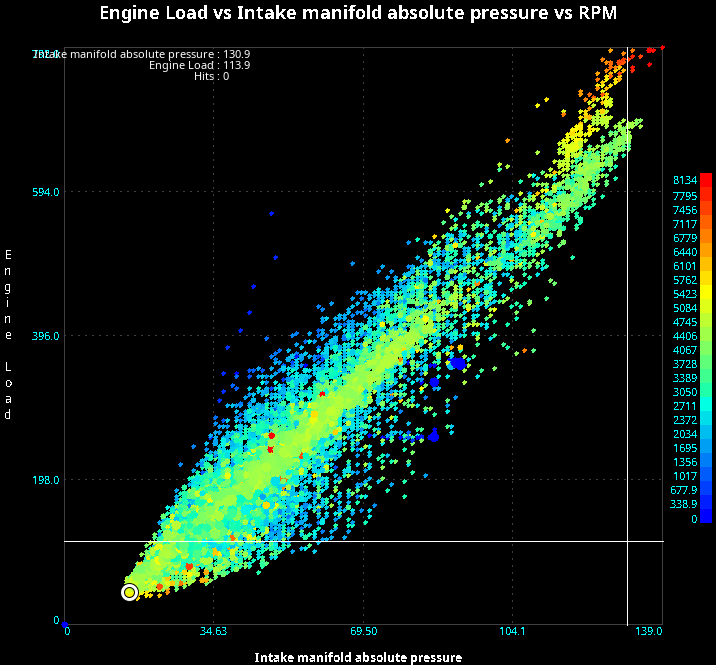
\includegraphics[max width=0.6\linewidth, keepaspectratio]{maf_map}
    \caption{Load vs.\ MAP scatter plot, coloured by RPM (MegaLogViewer HD).}
    \label{fig:maf_map}
\end{figure}

% =============================================================================
\section{Fuel Injection}
% =============================================================================

\subsection{Overview}

The injectors are driven by TPU-B channels 1--4 via a TLE6220GP quad low-side
switch. The ECU computes a pulse width in microseconds for each combustion
event.

\subsubsection*{Injector Dead Time}

The injector opening dead time (\texttt{CAL\_inj\_time\_base}, 2D vs battery voltage)
is added to the fuel
pulse width to compensate for the electrical delay before fuel actually flows.

\subsubsection*{Running Mode}

The running injection time is built up from several components:

\begin{enumerate}
	\item \textbf{Fuel load.} The air load (from MAF or Alpha-N) is divided
	      by the target AFR to obtain the fuel mass needed. The target AFR
	      comes from a 3D map (\texttt{CAL\_inj\_afr\_base}, indexed by RPM
	      and load). When the octane scaler (knock retard~2) is active,
	      the mixture is enriched proportionally via
	      \texttt{CAL\_inj\_afr\_adj\_per\_adv\_adj} to protect against
	      detonation.
	\item \textbf{Injector characteristics.} The fuel mass is converted to
	      pulse width using the injector flow rate
	      (\texttt{CAL\_inj\_flow\_rate}) and an efficiency map
	      (\texttt{CAL\_inj\_efficiency}, 3D vs RPM and load).
	\item \textbf{Corrections.} Three multiplicative adjustment factors are
	      applied:
	      \begin{itemize}
	      \item adj1: start enrichment (3D vs stop-coolant and accumulated
	            airflow),
	      \item adj2: intake air temperature correction (2D vs intake air temperature),
	      \item adj3: warm-up enrichment (3D vs load and coolant).
	      \end{itemize}
	\item \textbf{Transient enrichment.} Tip-in, tip-out, and DFSO reactive
	      enrichments are added (see Transient Fueling chapter).
	\item \textbf{Fuel trims.} The STFT and LTFT multiplicative corrections
	      are applied. The idle LTFT additive correction
	      (\texttt{LEA\_ltft\_zone1\_adj}, in microseconds) is added to the
	      final pulse width.
	\item \textbf{Evaporative fuel.} The estimated fuel vapour from the
	      charcoal canister purge is subtracted from the required fuel load
	      before computing the pulse width.
\end{enumerate}

The result is clamped to a minimum of 160\,$\mu$s. If the pulse width exceeds
the available time between combustion events, the duty cycle is reported as
100\,\% and the excess is carried forward.

\subsubsection*{Cranking Mode}

During cranking, a separate enrichment factor
(\texttt{CAL\_inj\_time\_adj\_cranking}, 2D vs coolant temperature at engine
stop) is applied on top of the dead time to provide the rich mixture needed for
starting.

\subsubsection*{DFSO (Decel Fuel Shut-Off)}

When the driver lifts off the throttle at speed, the ECU cuts fuel entirely.
DFSO engages when all conditions are met: engine speed above
\texttt{CAL\_dfso\_engine\_speed\_enable}, PPS below
\texttt{CAL\_dfso\_pps\_enable}, coolant above
\texttt{CAL\_dfso\_coolant\_enable}, and car speed above
\texttt{CAL\_dfso\_car\_speed\_enable}. Each condition has a separate
disable threshold with hysteresis for smooth re-engagement.

\subsubsection*{Rev Limiter}

The rev limiter cuts fuel by setting the fuel-cut flag when engine speed
exceeds a limit derived from \texttt{CAL\_revlimit\_speed\_base} (3D vs
coolant and a time-since-hit timer). When faults are present the limit is
reduced by \texttt{CAL\_revlimit\_speed\_adj\_limp\_reduced}. Launch control
can override with a lower limit (\texttt{LEA\_tc\_launchcontrol\_revlimit})
when the car is stationary.

\subsubsection*{Injection Angle}

The injection start angle relative to TDC is looked up
(\texttt{CAL\_inj\_angle}, 3D vs RPM and load). A development override
(\texttt{dev\_inj\_angle}) can replace it for testing.

\begin{landscape}
	\subsection{Running Mode}
	\formulagraph{dot/inj_running.pdf}{Injection time --- running mode}{fig:inj_running}

	\subsection{Fuel Load Detail}
	\formulagraph{dot/inj_fuel_load.pdf}{Fuel load calculation detail}{fig:inj_fuel_load}

	\subsection{Cranking Mode}
	\formulagraph{dot/inj_cranking.pdf}{Injection time --- cranking mode}{fig:inj_cranking}

	\subsection{DFSO (Decel Fuel Shut-Off)}
	\formulagraph{dot/inj_dfso.pdf}{DFSO enable/disable conditions}{fig:inj_dfso}

	\subsection{Rev Limiter}
	\formulagraph{dot/inj_revlimit.pdf}{Rev limiter --- fuel cut}{fig:inj_revlimit}
\end{landscape}

\subsection{Tuning Tips}

The most direct way to tune \texttt{CAL\_inj\_efficiency} is to log actual
versus target AFR over a representative drive and use MegaLogViewer~HD's
Histogram/Table generator to build a correction map, as shown in
Figure~\ref{fig:afr_log}. This requires a wideband AFR measurement --- either via the wideband patch
with a Spartan~2 controller exposing lambda over OBD, or any other valid
data-logging method that captures measured AFR alongside the ECU channels.

\subsubsection*{Axis Setup}

Set the X and Y axes in MegaLogViewer~HD to engine speed and load with the
same resolution as \texttt{CAL\_inj\_efficiency} (32 columns, 32 rows) and
the same breakpoint values. The resulting table then maps one-to-one onto the
calibration table, making corrections straightforward to transcribe.

\subsubsection*{Logging Strategy}

Log both the measured AFR from the wideband and the target AFR from the ECU.
Apply filters to exclude operating conditions where the base table should not
be evaluated:

\begin{itemize}
    \item \textbf{Transients}: exclude samples where \texttt{dt\_tps} exceeds
          a small threshold --- transient fuelling enrichments are handled
          separately and will pollute the steady-state map.
    \item \textbf{DFSO}: exclude samples during deceleration fuel cut-off.
    \item \textbf{Cold engine}: exclude samples below a minimum coolant
          temperature --- cold-start enrichments are not part of the
          efficiency table.
\end{itemize}

\subsubsection*{Correction Formula}

Work in lambda rather than AFR to keep the correction dimensionless and fuel
independent. The correction factor for each cell is the ratio of measured
lambda to target lambda: a value above~1 means the engine ran lean and the
efficiency value must be increased proportionally. To include the long-term
fuel trim already learned by the ECU, multiply by the active LTFT zone
correction. This combined factor can be entered directly in MegaLogViewer~HD
as a custom formula, producing a table whose values can be reported straight
into \texttt{CAL\_inj\_efficiency} without further arithmetic.

\begin{figure}[h]
    \centering
    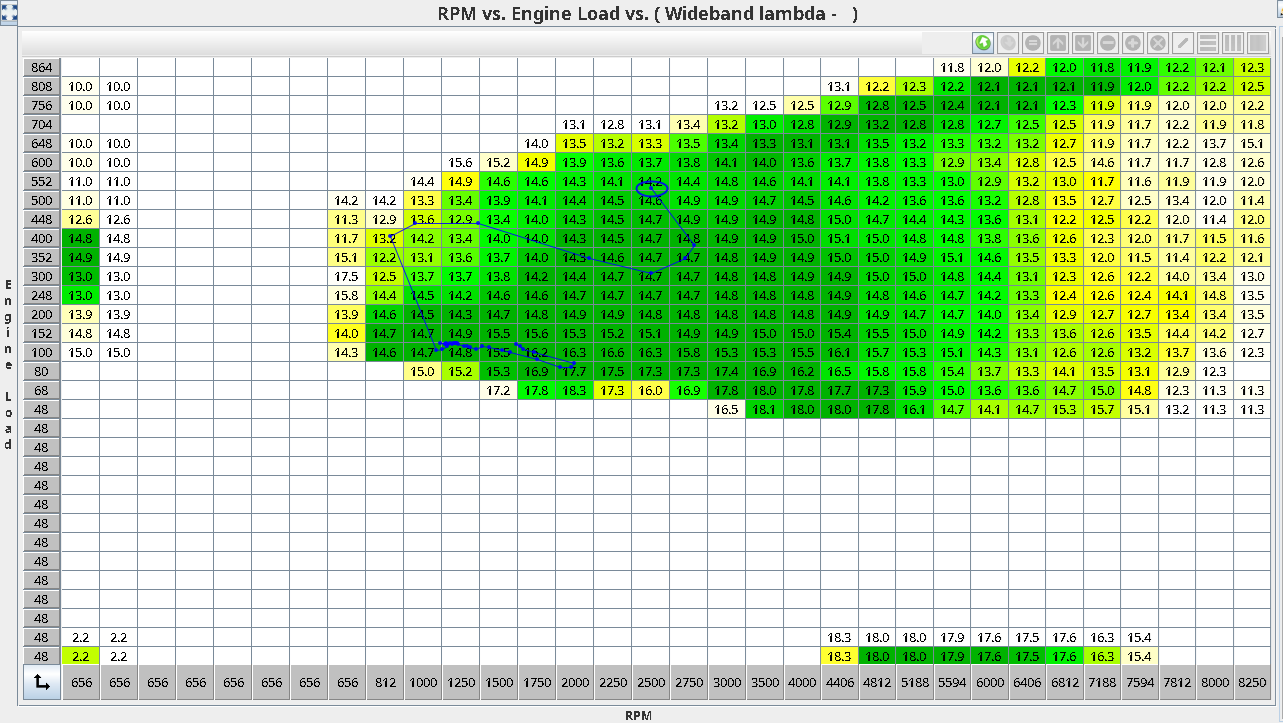
\includegraphics[max width=1.0\linewidth, keepaspectratio]{afr_log}
    \caption{Wideband AFR log --- MegaLogViewer~HD.}
    \label{fig:afr_log}
\end{figure}

\subsubsection*{Injector Duty Cycle}

The injectors must have enough headroom to deliver additional fuel when
enrichment is needed --- running close to 100\,\% duty cycle leaves no margin
for correction. Monitoring the duty cycle live is therefore important. It can be
computed from RPM (mode~\$01 PID~0x0C) and injection time
(mode~\$22 PID~\$0205). Many logging tools (OBD~Fusion, OBDLink, etc.) allow
combining PIDs in a custom formula, so this value can be displayed as a live
gauge without any post-processing.

% =============================================================================
\section{Transient Fueling}
% =============================================================================

\subsection{Overview}

The transient fueling system compensates for the fuel film dynamics that occur
during rapid throttle changes. Three independent enrichment terms are computed
and added directly to the injection pulse width (in microseconds). Closed-loop
fuel control is suspended while any enrichment is active.

\subsubsection*{TPS Rate Signal}

The core input is \texttt{dt\_tps\_injtip}, a peak-hold-with-decay version of
the throttle rate of change. Unlike the raw TPS derivative, this signal
captures the peak throttle movement and then decays gradually toward zero at a
calibrated rate (\texttt{CAL\_injtip\_in\_adj2} for positive,
\texttt{CAL\_injtip\_out\_adj2} for negative, both 2D vs RPM). A
threshold (\texttt{CAL\_injtip\_\{in,out\}\_dt\_tps\_target\_2\_min}) filters
small movements and a limit
(\texttt{CAL\_injtip\_\{in,out\}\_dt\_tps\_target\_2\_limit}) caps the maximum
magnitude. This
signal is also used by the ignition system for its transient advance
adjustment.

\subsubsection*{Tip-In Enrichment}

When \texttt{dt\_tps\_injtip} is positive (throttle opening), enrichment is
the product of the TPS rate, an engine speed adjustment (2D vs RPM), a coolant
adjustment (2D vs coolant temperature --- cold engines need more enrichment),
a per-gear factor (drivetrain inertia varies with gear ratio), and
\texttt{CAL\_injtip\_time\_base}.

\subsubsection*{Tip-Out Enrichment}

When \texttt{dt\_tps\_injtip} is negative (throttle closing), the magnitude is
negated and enrichment is calculated similarly but without the gear factor.
Despite the throttle closing, this is still an \emph{enrichment} (added to the
pulse width), maintaining combustion stability during the rapid transient.

\subsubsection*{DFSO and Reactive Enrichment}

Deceleration Fuel Shut-Off (DFSO) cuts fuel entirely when the engine is
decelerating with the throttle closed. Entry requires all of: engine speed
above threshold, sufficient runtime, coolant above minimum, and pedal below
threshold. A re-entry delay counter (looked up by PPS) prevents hunting at the
boundary. DFSO exits when engine speed drops below a lower threshold, pedal
is pressed, or coolant falls below minimum (all with hysteresis).

On DFSO exit, reactive enrichment protects the catalytic converter from the
lean exhaust accumulated during fuel cut.
The initial magnitude depends on how long DFSO was active
(\texttt{dfso\_count}), looked up from \texttt{CAL\_injtip\_catalyst\_adj}.
The enrichment then decays exponentially each combustion event, multiplied by
\texttt{CAL\_injtip\_catalyst\_adj\_fadeout} ($<1.0$) until it reaches zero.
Only then does closed-loop fuel control resume.

\begin{landscape}
	\subsection{Tip-In Enrichment}
	\formulagraph{dot/injtip_tip_in.pdf}{Tip-in enrichment formula}{fig:injtip_tip_in}

	\subsection{Tip-Out Enrichment}
	\formulagraph{dot/injtip_tip_out.pdf}{Tip-out enrichment formula}{fig:injtip_tip_out}

	\subsection{DFSO Reactive Enrichment}
	\formulagraph{dot/injtip_reactive.pdf}{DFSO reactive enrichment formula}{fig:injtip_reactive}
\end{landscape}

% =============================================================================
\section{Closed-Loop Fuel Control}
% =============================================================================

\subsection{Overview}

Closed-loop fuel control is active only when all of the following conditions
are met: the engine has been running longer than
\texttt{CAL\_stft\_runtime\_min} (which varies with coolant temperature
at stop), intake air temperature is above
\texttt{CAL\_stft\_engine\_air\_min}, the target AFR equals
stoichiometric (\texttt{CAL\_stft\_afr}), the pre-O2 sensor has been
validated (voltage has left the mid-range delimited by
\texttt{CAL\_stft\_o2\_test\_min} and \texttt{CAL\_stft\_o2\_test\_max} at least once), and there are no
active DFSO, transient enrichment, or traction control interventions.

When any of these conditions is not met, the ECU operates in open loop and the
STFT is held at zero.

\subsubsection*{Short-Term Fuel Trim (STFT)}

The STFT oscillates around stoichiometric based on the pre-O2 sensor voltage.
Two states exist: enriching (O2 below \texttt{CAL\_stft\_stoich\_min})
and enleaning (O2 above \texttt{CAL\_stft\_stoich\_max}).

On each O2 state transition, an initial jump is applied immediately, followed
by a gradual step added at a timed interval. Both the initial jump and the
step size come from 3D maps indexed by RPM and load, with separate maps for
enrichment and enleanment. At idle, dedicated scalar values are used instead,
and the step interval is scaled proportionally to engine speed so that the
trim advances synchronously with combustion events.

After a configurable time (\texttt{CAL\_stft\_time\_use\_adj}),
the step size is reduced by a factor
(\texttt{CAL\_stft\_enrichment\_step\_adj} and
\texttt{CAL\_stft\_enleanment\_step\_adj}) to slow
the oscillation once the trim has had time to converge.

The STFT is clamped to $\pm$\texttt{CAL\_stft\_limit}.

\subsubsection*{Long-Term Fuel Trim (LTFT)}

The LTFT learns persistent fueling errors from a low-pass filtered version of
the STFT (\texttt{inj\_time\_stft\_smooth}, filtered with
\texttt{CAL\_stft\_smooth\_reactivity}). If the smoothed STFT
stays consistently above or below calibrated thresholds, the LTFT is stepped
in the corresponding direction.

Four zones exist, selected by MAF airflow:

\begin{description}
	\item[Zone 1] Below \texttt{CAL\_ltft\_zone1\_flow\_max}
	      and RPM below
	      \texttt{CAL\_ltft\_zone1\_engine\_speed\_max}.
	      The correction (\texttt{LEA\_ltft\_zone1\_adj}) is \emph{additive}
	      in microseconds, stepped by
	      \texttt{CAL\_ltft\_zone1\_step}.
	\item[Zone 2] Between the zone1 and zone2-max flow thresholds, with load
	      within a defined window. The correction
	      (\texttt{LEA\_ltft\_zone2\_adj}) is \emph{multiplicative}.
	\item[Mid] Between the low-max and high-min flow thresholds. The
	      multiplicative correction is linearly interpolated between the low
	      and high learned values based on the current MAF position within
	      the range.
	\item[Zone 3] Above \texttt{CAL\_ltft\_zone3\_flow\_min}.
	      The correction (\texttt{LEA\_ltft\_zone3\_adj}) is
	      \emph{multiplicative}.
\end{description}

Even when the ECU is in open loop (STFT inactive), the LTFT corrections are
still applied to the injection pulse width --- only the learning (stepping of
the learned values) is suspended. This means the ECU always benefits from
previously learned fuel corrections regardless of operating mode.

LTFT learning is further gated by: coolant and intake air temperature above
minimum thresholds, atmospheric pressure above
\texttt{CAL\_ltft\_atmo\_min}, fuel level above
\texttt{CAL\_ltft\_fuel\_min}, and no evaporative system pressure
drop in progress. The update interval is controlled by
\texttt{CAL\_ltft\_time\_between\_step}. Each zone has independent
limits.

\begin{landscape}
	\subsection{Short-Term Fuel Trim (STFT)}	
	\formulagraph{dot/stft.pdf}{STFT formula}{fig:stft}

	\subsection{Long-Term Fuel Trim (LTFT)}
	\formulagraph{dot/ltft.pdf}{LTFT formula}{fig:ltft}
\end{landscape}

\subsection{Tuning Tips}

Figure~\ref{fig:ltft_cup260} shows the \texttt{CAL\_inj\_afr\_base} table from a
Lotus Exige~S Cup~260 calibration, colorized by the active LTFT zone at each
cell. The colour coding matches the zone boundaries defined by the flow and load
thresholds described above: \textbf{blue} for Zone~1 (idle), \textbf{green} for
Zone~2 (part-load), \textbf{pink} for Zone~3 (high-load), and \textbf{yellow}
for the dead zone between Zone~2 and Zone~3 where the two corrections are
interpolated. Bold values mark cells calibrated to the stoichiometric target
(14.6~AFR), meaning the ECU will run in closed loop at those points and the STFT
can drive LTFT learning.

A key design constraint is that \emph{each zone must contain enough cells
at~14.6} to give the ECU sufficient closed-loop operating time to build a
reliable correction for that zone. A zone with too few stoichiometric cells will
rarely enter closed loop there, leaving its learned correction at the reset
default and therefore inaccurate. As the figure illustrates, the Cup~260
calibration provides wide stoichiometric coverage across all three zones:
the entire idle region (Zone~1), a broad part-load band (Zone~2), and a
high-load band before the enrichment ramp begins (Zone~3).

\textbf{Zone~3 correction applies at WOT.} At wide-open throttle the AFR target
drops well below stoichiometric, the STFT is suspended and the ECU enters open
loop --- but \texttt{LEA\_ltft\_zone3\_adj} is still applied multiplicatively to
the base injection time. A miscalibrated Zone~3 LTFT therefore directly affects
WOT fuelling, even though no learning takes place there. \textbf{It is essential
that the Zone~3 stoichiometric cells in the AFR table are reachable under normal
part-throttle driving so that the ECU can converge on the correct correction
before it is relied upon at full load.}

\textbf{Note:} this is one of the most commonly overlooked aspects of closed-loop
fuel tuning. A competent tuner should produce exactly this kind of Excel Sheet
--- overlaying the AFR targets with the LTFT zone boundaries --- to verify that
each zone, and Zone~3 above all, has sufficient stoichiometric coverage for
learning to occur. In practice, many tuners focus exclusively on the WOT
enrichment values and never verify Zone~3 LTFT convergence. Some are not even
aware that the Lotus ECU operates with multiple independent LTFT zones at all.

\begin{landscape}
	\formulagraph[page=1]{ltft_cup260.pdf}{AFR Target - Learning Zones (Lotus Exige S Cup 260)}{fig:ltft_cup260}
\end{landscape}

% =============================================================================
\section{Ignition}
% =============================================================================

\subsection{Overview}

The engine uses four individual ignition coils (coil-on-plug). Dwell and fire
timing are handled in hardware by TPU-A channels 1--4; the main CPU only
computes advance angles and dwell duration.

\subsubsection*{Dwell Time}

The dwell time is looked up from a 3D table indexed by engine speed and battery
voltage (\texttt{CAL\_ign\_dwell\_base}). At high RPM, if the required dwell
would overlap the previous cylinder's fire event, the dwell is shortened
automatically.

\subsubsection*{Operating Modes}

The ECU selects one of four ignition modes based on engine state:

\begin{description}
	\item[Cranking] A simple 2D vs coolant temperature at the time the
	      engine was stopped. Active for
	      \texttt{CAL\_ign\_cranking\_runtime\_max} after the engine starts.
	\item[Running] Full advance calculation: base map plus adjustments for
	      intake air temperature, transient throttle, RPM, and accumulated
	      airflow. Two base maps exist (low cam and high cam) and the correct
	      one is selected by the current VVL state.
	\item[Idle] A separate formula based on coolant temperature, idle speed
	      error, and rate of change of engine speed. Includes an AC compressor
	      offset.
	\item[DFSO] A single fixed advance value (\texttt{CAL\_ign\_adv\_dfso}),
	      bypassing the normal calculation entirely.
\end{description}

\subsubsection*{Per-Cylinder Final Stage}

After the mode-specific formula produces a final advance value, a 5\,ms
smoothing task ramps the advance in configurable steps (sized by RPM and PPS)
to avoid abrupt timing changes. The smoothed value then passes through a
per-cylinder stage that applies:

\begin{itemize}
	\item A per-cylinder trim offset (\texttt{CAL\_ign\_adv\_adj\_cyl}).
	\item Knock retard~1: immediate timing retard from the knock detection
	      system, recovered gradually in the post-fire ISR phase.
	\item Knock retard~2 (octane scaler): a long-term learned factor
	      (0--100\,\%) per cylinder that blends the base ignition map with
	      a conservative knock-safe map (low octane map).
\end{itemize}

The result is clamped to \texttt{CAL\_ign\_adv\_limit\_l} and loaded into
the TPU parameters for hardware-timed execution.

\begin{landscape}
	\subsection{Running Mode}
	\formulagraph{dot/ign_running.pdf}{Ignition advance --- running mode}{fig:ign_running}

	\subsection{Per-Cylinder Final Stage}
	\formulagraph{dot/ign_percyl.pdf}{Ignition advance --- per-cylinder final stage}{fig:ign_percyl}

	\subsection{Idle Mode}
	\formulagraph{dot/ign_idle.pdf}{Ignition advance --- idle mode}{fig:ign_idle}

	\subsection{Cranking Mode}
	\formulagraph{dot/ign_cranking.pdf}{Ignition advance --- cranking mode}{fig:ign_cranking}

	\subsection{DFSO Mode}
	\formulagraph{dot/ign_dfso.pdf}{Ignition advance --- DFSO mode}{fig:ign_dfso}

	\subsection{Traction Control Retard}
	\formulagraph{dot/ign_tc.pdf}{Ignition retard from traction control}{fig:ign_tc}
\end{landscape}

\subsection{Tuning Tips}

The high-cam ignition map (3D vs RPM and load) is only used when VVL is
engaged \emph{and} RPM is below \texttt{CAL\_vvl\_rpm\_enable} \emph{and}
load is above \texttt{CAL\_vvl\_high\_load\_enable}. In all other
cases --- including high cam at high RPM --- the low-cam map (also 3D vs
RPM and load) is used.

On the Elise, \texttt{CAL\_vvl\_rpm\_high\_load\_enable} is set
to the same value as \texttt{CAL\_vvl\_rpm\_enable}, which means VVL can only
engage at the normal RPM threshold and the high-cam ignition map is
effectively never used. The same applies to its knock-safe variant.
The original Elise calibration contains garbage values in both tables
(\texttt{CAL\_ign\_adv\_high\_cam\_base} and
\texttt{CAL\_ign\_adv\_high\_cam\_knock\_safe}). If you lower
\texttt{CAL\_vvl\_rpm\_high\_load\_enable} to engage VVL earlier under high
load, both high-cam maps \emph{will} be used in the RPM range between
\texttt{CAL\_vvl\_rpm\_high\_load\_enable} and \texttt{CAL\_vvl\_rpm\_enable}
--- populate them with correct values first. Garbage values in this range will
cause a dramatic and sudden power loss that resembles a rev limiter firing
between the two threshold RPMs.

The ignition advance reported over the standard OBD interface (PID~\$0E) is
\texttt{ign\_adv\_final}, which is computed before the per-cylinder final
stage. Per-cylinder trim (\texttt{CAL\_ign\_adv\_adj\_cyl}), knock retard~1
and knock retard~2 (octane scaler) are all applied \emph{after} this value is
set. This means that any knock-induced retard is invisible to a standard OBD
logger --- the displayed advance will look clean even while the ECU is
actively pulling timing on individual cylinders.

Figure~\ref{fig:tuner} shows a live-tuning tool in use on a dyno. The ignition
advance table is displayed with the cell currently active highlighted in
real time, allowing timing to be increased or decreased on the fly using the
keyboard. The octane scalers are visible alongside, giving an immediate view
of knock activity on each cylinder. AFR can also be monitored precisely when
the wideband patch is applied and a Spartan~2 wideband controller is connected.

\begin{figure}[h]
    \centering
    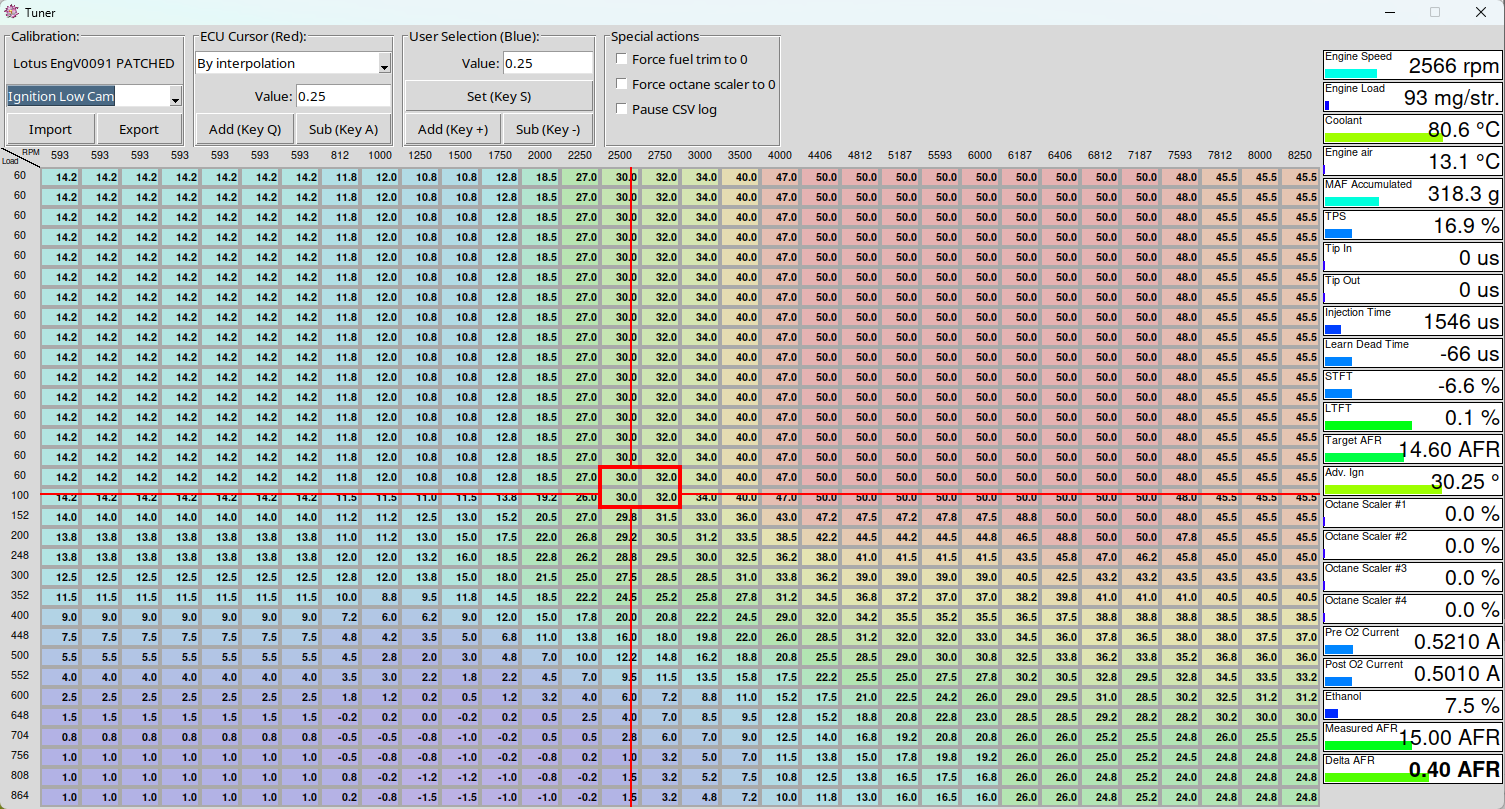
\includegraphics[max width=\linewidth, keepaspectratio]{tuner}
    \caption{Live ignition map editing over CAN-Bus RAM access on a dyno.}
    \label{fig:tuner}
\end{figure}

\subsection{Igniter Feedback (IGF)}

The ECU uses the IGF (Igniter Feedback) signal from the ignition coil pack
to confirm that each coil fired successfully.

Each ignition event generates three TPU-A interrupts per cylinder:

\begin{enumerate}
	\item \textbf{Dwell start.}
	      The TPU channel function status reaches 0xE, indicating the crank
	      angle for dwell onset. The ISR programs the dwell duration and
	      resets its phase counter.

	\item \textbf{Fire.}
	      The phase counter is below~2 (first two non-dwell interrupts).
	      The ISR sets a pending-feedback bit for this cylinder. Before
	      doing so, it checks whether any \emph{other} cylinders' pending
	      bits are still set --- meaning those coils fired but their IGF
	      confirmation never arrived. Those cylinders are flagged in a
	      separate missed-feedback register.

	\item \textbf{Post-fire.}
	      The phase counter reaches~2 and is reset. The knock retard~1
	      recovery timer for this cylinder is processed (see Knock
	      Detection), and the next ignition event is scheduled.
\end{enumerate}

The IGF signal is received on TPU-B channel~15. When the interrupt fires,
it clears the pending-feedback bit for the cylinder that most recently
fired. If the bit is cleared before the next cylinder's fire phase, the
coil is confirmed working.

Every 200\,ms, \texttt{misfire\_monitor\_200ms} evaluates the
missed-feedback register. Each cylinder's bit is fed into a diagnostic
channel with confirm/clear thresholds. Once a fault is confirmed the
corresponding DTC is set:

\begin{description}
	\item[P0351] Ignition coil A primary/secondary circuit.
	\item[P0352] Ignition coil B primary/secondary circuit.
	\item[P0353] Ignition coil C primary/secondary circuit.
	\item[P0354] Ignition coil D primary/secondary circuit.
\end{description}

Both the pending-feedback and missed-feedback registers are cleared when
the engine stops.

\subsection{Combustion Misfire Detection}

Separate from the IGF coil-failure check, the ECU detects actual combustion
misfires by monitoring the time each cylinder takes to complete its power
stroke. A misfiring cylinder produces a longer stroke period than its
neighbours because the piston is not driven by combustion pressure.

\subsubsection*{Detection Pipeline}

At every TDC event the crank-position ISR processes each cylinder in firing
order (1, 3, 4, 2) through three successive stages that progressively isolate
the misfire signal from noise:

\begin{enumerate}
  \item \textbf{Smoothing.} A mild filter removes the effect of RPM
        acceleration between consecutive strokes of the same cylinder, giving a
        smoothed stroke time (\texttt{misfire\_stroke\_time\_smooth}).

  \item \textbf{Inter-cylinder difference.} The smoothed stroke time of the
        current cylinder is subtracted from the raw stroke time of the previous
        cylinder in the firing sequence (\texttt{misfire\_stroke\_cyl\_diff}).
        This removes the absolute stroke duration and leaves only the
        relative variation between adjacent cylinders.

  \item \textbf{Baseline correction.} A 16$\times$4 learned table
        (\texttt{LEA\_misfire\_stroke\_time}, one row per RPM band, one column
        per cylinder) captures the normal inter-cylinder variation for this
        specific engine. Subtracting the table value gives the residual
        deviation (\texttt{misfire\_stroke\_diff\_1}). The table is adapted
        continuously during DFSO, slowly tracking natural stroke-time asymmetry
        between cylinders.

  \item \textbf{Adjacent-cylinder normalisation.} The residual of the previous
        cylinder is subtracted from the current residual
        (\texttt{misfire\_stroke\_diff\_2}). This cancels any engine-wide RPM
        disturbance that affects all cylinders equally, leaving a signal
        sensitive only to single-cylinder anomalies.
\end{enumerate}

\subsubsection*{Two-Tier Thresholds}

Two independent thresholds are applied at each TDC event:

\begin{description}
  \item[Emission misfire] The baseline-corrected residual
        (\texttt{misfire\_stroke\_diff\_1}) is compared against
        \texttt{misfire\_threshold}. Events are counted per cylinder over a
        rolling window of 2000 strokes; at the end of each window the counts
        are halved and stored in \texttt{LEA\_misfire\_count}. Sustained rates
        above the OBD limits set P0301--P0304.

  \item[Catalyst-damage misfire] The normalised residual
        (\texttt{misfire\_stroke\_diff\_2}) is compared against
        \texttt{misfire\_cat\_threshold}. A per-cylinder countdown timer
        (\texttt{misfire\_cat\_timer}) decrements each time the threshold is
        exceeded and resets to \texttt{misfire\_cat\_timer\_max} otherwise. A
        separate 400-stroke window accumulates \texttt{misfire\_cat\_count}.
        The normalised signal is used here because single severe misfires must
        be detected even when global RPM is fluctuating.
\end{description}

\subsubsection*{Array Index Order}

All misfire arrays follow firing order: index~0 = cylinder~1, index~1 =
cylinder~3, index~2 = cylinder~4, index~3 = cylinder~2. The OBD dev-mode PIDs
\$0234--\$0237 report \texttt{misfire\_count[0..3]} in the same order
(see Table~\ref{tab:mode22}).

% =============================================================================
\section{Knock Detection}
% =============================================================================

\subsection{Overview}

Understanding the knock noise baseline for your specific engine setup is
essential before tuning ignition timing aggressively.

\subsubsection*{Hardware and Signal Processing}

A piezoelectric knock sensor is mounted on the engine block. The signal is
band-pass filtered and amplified by the L9119D knock IC, then read from
QADC-B and compared to an exponentially-smoothed baseline (per cylinder). The
peak ratio is computed as \texttt{knock\_signal * 10 / (baseline + 1)}.
When the ratio exceeds \texttt{CAL\_knock\_peak\_threshold} (3D vs RPM
and load), knock is detected and the excess above the threshold is recorded
as a severity measure (\texttt{knock\_peak\_over\_threshold}).

The sensor amplifier gain is configured per cylinder via SPI, using four
independent maps (\texttt{CAL\_knock\_sensitivity\_cylinder1\ldots4},
each 3D vs RPM and load). When knock is not detected, the baseline
tracks the signal via \texttt{CAL\_knock\_signal\_reactivity}; when knock is
detected, the baseline is raised by \texttt{CAL\_knock\_signal\_fadeout\_step}
to prevent the same event from re-triggering.

\subsubsection*{Knock Window}

The crank angle window during which the sensor signal is sampled is defined by
two maps: \texttt{CAL\_knock\_window\_start} and
\texttt{CAL\_knock\_window\_width} (both 3D vs RPM and load). A
minimum width of 5\textdegree{} is enforced. The window parameters are computed
per cylinder and loaded into the TPU for hardware-timed acquisition.

\subsubsection*{Enable Conditions}

Knock retard is only active when all of the following are met:
\begin{itemize}
\item Engine load above \texttt{CAL\_knock\_retard\_load\_min} (2D vs speed,
      with hysteresis via \texttt{CAL\_knock\_load\_margin}).
\item Engine speed within
      \texttt{CAL\_knock\_retard1\_engine\_speed\_min\ldots max}
      (with hysteresis via \texttt{CAL\_knock\_speed\_margin}).
\item Coolant temperature above \texttt{CAL\_knock\_retard1\_coolant\_min}.
\item VVT deviation within \texttt{CAL\_knock\_retard1\_vvt\_diff\_max}
      (avoids false detection during cam phasing transients).
\item TPS transient blanking timer expired --- rapid throttle changes
      (\texttt{dt\_tps\_target\_2} exceeding
      \texttt{CAL\_knock\_retard1\_dt\_tps\_target\_2\_max})
      blank detection for \texttt{CAL\_knock\_retard1\_dt\_tps\_target\_2\_time}.
\end{itemize}
When any condition is lost, retard1 is cleared immediately.

\subsubsection*{Retard 1 --- Immediate Retard}

On knock detection, \texttt{knock\_retard1} is increased by a value looked up
from \texttt{CAL\_knock\_retard1\_inc} (indexed by knock severity), clamped to
\texttt{CAL\_knock\_retard1\_limit}. This is tracked per cylinder.

Recovery is paced by \texttt{CAL\_knock\_retard1\_time\_between\_step}
(counted down in 50\,ms increments): each time the timer reaches zero, the
post-fire ISR decrements retard1 by \texttt{CAL\_knock\_retard1\_dec} and
reloads the timer. This repeats until retard1 reaches zero. If new knock is
detected during recovery, retard1 is increased again and the timer restarts.

\subsubsection*{Retard 2 --- Long-Term Octane Adaptation}

Lotus calls this correction the \emph{Octane Scaler}. Its purpose is to
adapt timing to the octane rating of the fuel in the tank: the knock-safe
map can therefore be thought of as a \emph{low-octane} ignition table ---
the timing schedule the ECU falls back to when running on poor-quality fuel.

\texttt{LEA\_knock\_retard2[0\ldots3]} is a per-cylinder learned factor
(0--100\,\%) that blends the base ignition map toward the knock-safe map.
It is persisted in EEPROM across power cycles.

When retard1 is active (knock occurring), \texttt{LEA\_knock\_retard2} increases
proportionally to retard1 via \texttt{CAL\_knock\_retard2\_corr\_inc\_coef}.
When retard1 is zero (no knock), it slowly decays by
\texttt{CAL\_knock\_retard2\_corr\_dec\_step}. This makes the ECU
progressively retard timing for cylinders that repeatedly knock, adapting to
fuel quality and engine condition.

The actual retard2 applied is the learned fraction of the difference between
the base ignition map and the knock-safe map. Retard2 learning requires load
above a separate threshold (\texttt{CAL\_knock\_retard2\_corr\_load\_min}).

\begin{landscape}
	\subsection{Knock Retard 1 --- Immediate Retard}
	\formulagraph{dot/knock_retard1.pdf}{Knock retard 1 --- immediate retard and recovery}{fig:knock_retard1}

	\subsection{Knock Retard 2 --- Octane Learned Factor}
	\formulagraph{dot/knock_retard2.pdf}{Knock retard 2 --- octane learned factor}{fig:knock_retard2}
\end{landscape}

\subsection{Tuning Tips}

Calibrating \texttt{CAL\_knock\_peak\_threshold} is a chicken-and-egg problem:
you need to drive the car to measure the sensor signal level, but if the
thresholds are wrong you risk either masking real knock or triggering false
retard events that corrupt the data.

This problem is compounded on supercharged variants. The supercharger
introduces broadband mechanical noise that the knock sensor picks up across the
entire RPM range, leaving less margin to distinguish genuine detonation from
background noise. A smaller supercharger pulley spins the blower faster and
raises the noise floor further, making threshold calibration even more
critical on high-boost builds.

A reliable approach is to eliminate any possibility of real knock during the
calibration drive, then treat every above-threshold event in
\texttt{knock\_peak\_over\_threshold} as background noise to be characterised.
This can be achieved by:

\begin{itemize}
    \item Filling the tank with a high-ethanol blend or a very high octane
          fuel. Both give a large margin against detonation even under
          aggressive conditions.
    \item Using a conservative, knock-safe ignition map for the session --- the
          goal is sensor characterisation, not performance.
\end{itemize}

With knock ruled out by chemistry and timing, \texttt{knock\_peak\_over\_threshold}
can be monitored in real time. Two options exist to expose it during the drive:

\begin{itemize}
    \item \textbf{Live-tuning access} (Section~\ref{sec:live-tuning}): poll the
          variable directly over CAN-Bus without any firmware modification.
          This is the simplest approach on unlocked ECUs.
    \item \textbf{Software patch}: redirect the peak-over-threshold value into
          an OBD-accessible location, allowing standard OBD logging tools to
          record it alongside all other channels.
\end{itemize}

Driving the full RPM and load range then yields a clean map of the sensor noise
floor across all operating points --- exactly the baseline needed to set
\texttt{CAL\_knock\_peak\_threshold} correctly: high enough to reject noise,
low enough to catch real knock the moment it occurs.

Note that \texttt{knock\_peak\_over\_threshold} is a four-element array, one
entry per cylinder. Significant differences between cylinders during the
characterisation drive indicate that the sensor signal level varies from one
cylinder to another --- due to mechanical tolerances, sensor mounting
position, or combustion chamber differences. In that case the per-cylinder
sensitivity tables (\texttt{CAL\_knock\_sensitivity\_cylinder1} through
\texttt{CAL\_knock\_sensitivity\_cylinder4}) should be adjusted individually
to bring all four readings into the same range before the threshold table is
finalised.

Figure~\ref{fig:knock_baseline} shows an example baseline for cylinder~3
logged on a Lotus Exige S Cup~260, visualised in MegaLogViewer~HD using the
Histogram/Table generator with the same RPM and load axes as
\texttt{CAL\_knock\_peak\_threshold}.
Figure~\ref{fig:knock_threshold_cup260} shows the original
\texttt{CAL\_knock\_peak\_threshold} from the same car, as a starting point
for comparison.

\begin{figure}[h]
    \centering
    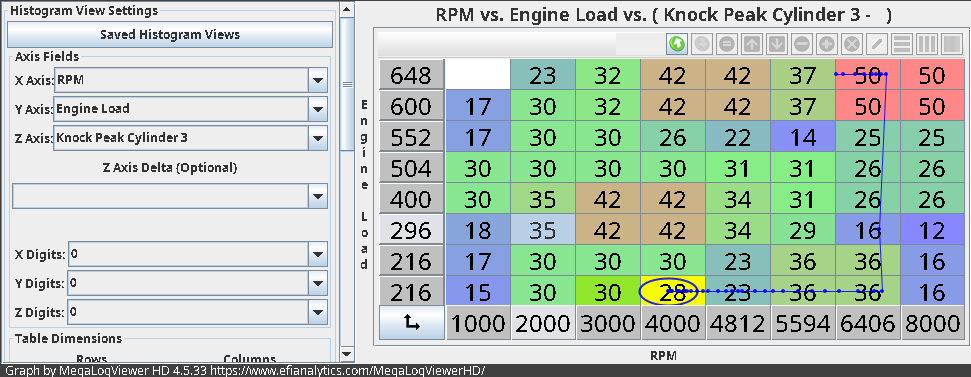
\includegraphics[max width=\linewidth, keepaspectratio]{knock_baseline}
    \caption{Cylinder~3 noise floor baseline --- MegaLogViewer HD (Lotus Exige S Cup~260).}
    \label{fig:knock_baseline}
\end{figure}

\begin{figure}[h]
    \centering
    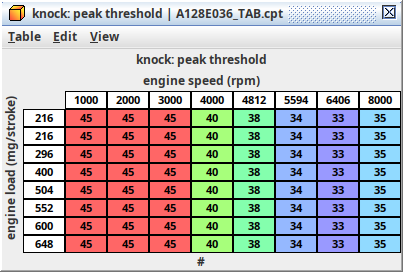
\includegraphics[max width=\linewidth, keepaspectratio]{peak_threshold_cup260}
    \caption{\texttt{CAL\_knock\_peak\_threshold} --- Lotus Exige S Cup~260 original calibration.}
    \label{fig:knock_threshold_cup260}
\end{figure}

% =============================================================================
\section{Idle Control}
% =============================================================================

\subsection{Overview}

The idle control system operates in the airflow domain: it computes a target
air mass flow (mg/s) rather than a throttle angle directly. The flow target is
then converted to a TPS position via lookup tables, and added to the pedal
demand in the throttle control stage.

\subsubsection*{Speed Target}

The idle speed target is the sum of:
\begin{itemize}
\item \textbf{Base idle speed} --- 2D vs coolant temperature
      (\texttt{CAL\_idle\_speed\_base}). Cold engines idle higher.
\item \textbf{Vehicle speed adjustment} --- 2D vs car speed
      (\texttt{CAL\_idle\_speed\_adj}). Raises idle when moving. Ramps down
      slowly via \texttt{CAL\_idle\_speed\_time\_between\_decrement} when the
      condition clears.
\item \textbf{AC compressor} --- additive offset
      (\texttt{CAL\_idle\_speed\_adj\_ac\_on}) when the AC is running.
\end{itemize}
The total is clamped to 1\,520\,rpm. The speed error
(\texttt{engine\_speed\_idle\_error}) is the difference between actual and
target speed, used by the flow adjustments below.

\subsubsection*{Flow Target}

The flow target is computed as the base flow plus a large number of
signed adjustments:
\begin{itemize}
\item \textbf{adj1} (learned, \texttt{LEA\_idle\_flow\_adj1}) --- long-term
      learned correction persisted in EEPROM. Separate values for AC
      on/off. See learning section below.
\item \textbf{adj2} --- atmospheric pressure correction (2D vs atmo),
      subtracted from the total.
\item \textbf{adj3} --- battery voltage compensation (2D vs voltage, signed).
      Low voltage increases airflow to raise alternator output.
\item \textbf{adj4 $\times$ adj4\_adj} --- feed-forward compensation based on
      the speed target itself (2D vs target idle), scaled by a 3D adjustment
      (coolant $\times$ accumulated air mass).
\item \textbf{adj5} --- proportional term (2D vs speed error, signed). Only
      active when the pedal is below \texttt{CAL\_idle\_flow\_pps\_max}
      and vehicle speed is below \texttt{CAL\_idle\_flow\_adj5\_max}
      (or engine speed is below target).
\item \textbf{adj6} --- vehicle speed compensation (2D vs car speed).
\item \textbf{adj7} --- dashpot (2D vs RPM). When engine speed
      exceeds the idle target by \texttt{CAL\_idle\_flow\_adj7\_enable},
      this adds extra airflow to cushion the deceleration back to idle. Phased
      out linearly below \texttt{CAL\_idle\_flow\_adj7\_disable}.
\item \textbf{adj8} --- integrator. Accumulates correction based on speed
      error every \texttt{CAL\_idle\_flow\_adj8\_corr\_time\_between\_step},
      clamped by calibrated limits. Drives the long-term learning (adj1).
\item \textbf{adj ac} --- ramp-up offset when the AC compressor engages
      (\texttt{CAL\_idle\_flow\_adj\_ac}, 2D vs time since AC on).
\item \textbf{adj fan} --- separate offsets for low-speed and
      high-speed cooling fans
      (\texttt{CAL\_idle\_flow\_adj\_fan\_low/high}, each 2D vs time since
      fan on).
\item \textbf{Evap purge} --- the estimated canister purge flow is subtracted,
      since purge air displaces throttle air.
\end{itemize}

\subsubsection*{Long-Term Learning (adj1)}

The integrator (adj8) acts as the fast correction. When adj8 consistently
deviates beyond \texttt{CAL\_idle\_flow\_adj1\_corr\_max/min},
the learned value \texttt{LEA\_idle\_flow\_adj1} is incremented or decremented
by one unit. This slowly transfers the integrator's correction into the
long-term learned value, so the integrator can remain near zero for the next
idle event. Separate learned values are maintained for AC on
(\texttt{LEA\_idle\_flow\_adj1\_ac\_on}) and off. Learning requires
sufficient engine run-time (\texttt{CAL\_idle\_flow\_adj1\_corr\_maf\_accumulated\_min})
and is suspended during evap purge.

\subsubsection*{Flow to TPS Conversion}

The flow target is converted to a throttle position for the motor controller:
\begin{itemize}
\item \textbf{Engine running} --- lookup (\texttt{CAL\_idle\_tps},
      3D vs flow target and intake vacuum), clamped to
      \texttt{CAL\_idle\_tps\_limit\_h}.
\item \textbf{Engine stopped} --- lookup
      (\texttt{CAL\_idle\_tps\_engine\_stop}, 3D vs atmospheric pressure and
      coolant temperature). This pre-positions the throttle for starting.
\end{itemize}
The resulting \texttt{idle\_tps\_target} is then added to the pedal-demand
TPS in the throttle control section.

\subsubsection*{Interaction with Ignition}

When the idle flag is set (PPS below threshold and engine speed below the
disable threshold), the ignition system switches from the running advance maps
to dedicated idle advance maps with their own base, speed error correction,
and rate-of-change damping.

\begin{landscape}
	\subsection{Speed Target}
	\formulagraph{dot/idle_speed_target.pdf}{Idle speed target calculation}{fig:idle_speed_target}
\end{landscape}

\begin{landscape}
	\subsection{Flow Target}
	\formulagraph{dot/idle_flow_target.pdf}{Idle flow target}{fig:idle_flow_target}
\end{landscape}

% =============================================================================
\section{Throttle Control}
% =============================================================================

\subsection{Overview}
The throttle target is the sum of the pedal demand and the idle air contribution,
clamped to calibration limits and ramped for smooth actuation.

\subsection{Throttle Body Startup Sequence}

At power-on, before the engine can be cranked, the ECU runs a state machine that
verifies the throttle body is mechanically sound. The sequence is driven by the
QADC interrupt (each ADC conversion cycle triggers one state machine step):

\begin{enumerate}
	\item \textbf{Motor off (state 0).}
	      The H-bridge PWM is set to zero and the motor enable is configured so
	      the throttle blade is released. A delay counter of 100 ADC cycles is
	      loaded, giving the return spring time to pull the blade to its rest
	      position.

	\item \textbf{ADC capture (state 1).}
	      The counter from state~0 decrements each cycle. When it reaches zero
	      the raw TPS1 ADC value is captured. This is the spring-rest voltage
	      with no motor drive applied.

	\item \textbf{Spring test / PID drive (state 2).}
	      The PID controller begins driving the throttle toward
	      an initial target of $\approx$\,0.71\,V (hardcoded). Once the position error falls
	      below~29\,mV, the setpoint is moved to fully closed
	      ($\approx$\,0.59\,V raw ADC, hardcoded in program code). The motor
	      must push the throttle closed against the return spring past the
	      spring rest position ($\approx$\,18.5\%), verifying motor authority.
	      A stability check loop then begins: every 10 cycles a snapshot of
	      the TPS voltage is taken, and 9 cycles later the snapshot is
	      compared with the current voltage. While the PID is still driving
	      the throttle closed, the position is changing and the check
	      naturally fails. The loop repeats until:
	      \begin{itemize}
	      \item \emph{Pass:} the voltage has not moved more than
	            $\pm$15\,mV since the last snapshot --- the throttle has
	            settled at the target. The state machine advances to
	            calibration.
	      \item \emph{Fail:} the timeout (1000 ADC cycles, hardcoded) expires before
	            the position stabilizes. The
	            \texttt{tps\_state\_test\_failed} flag is set and the machine
	            jumps directly to state~4 (active control), skipping
	            calibration. This flag causes \textbf{P0638} (Throttle
	            Actuator Control Range/Performance) to be set the next time
	            the diagnostic monitor runs.
	      \end{itemize}

	\item \textbf{Sensor calibration (state 3).}
	      Using the motor-driven closed voltage from state~2:
	      \begin{itemize}
	      \item For each sensor (TPS1, TPS2): the closed voltage is compared
	            with the calibration default
	            (\texttt{CAL\_sensor\_tps\_\{1,2\}\_offset}). If within
	            $\pm$0.1\,V, the learned offset
	            (\texttt{LEA\_sensor\_tps\_\{1,2\}\_offset}) is blended 50\%
	            toward the measurement. Otherwise it is reset to the
	            calibration default.
	      \item The corrected range and gain for both sensors are recomputed.
	      \item The motor is turned off and the machine advances to state~4.
	      \end{itemize}

	\item \textbf{Active motor control (state 4).}
	      Normal throttle control begins: the target is computed from PPS demand
	      plus idle contribution, clamped and ramp-smoothed (see TPS Target
	      below).
\end{enumerate}

\subsubsection*{Fault Mode Behavior}

During active control (state~4), if any fault flag is set --- including the
startup test failure flag, TPS sensor faults, or HC08 disagreement --- the motor
PWM is forced to zero, the H-bridge is disabled, and the throttle falls back to
its spring-rest position. The HC08 is also notified via the forced-idle flag.

\subsubsection*{Related OBD Diagnostic Codes}

\begin{description}
	\item[P0122] TPS1 circuit low input (ADC below range).
	\item[P0123] TPS1 circuit high input (ADC above range).
	\item[P0222] TPS2 circuit low input (ADC below range).
	\item[P0223] TPS2 circuit high input (ADC above range).
	\item[P0638] Throttle actuator control range/performance --- the throttle
	      position does not track the target. Set when the position error
	      (\texttt{tps\_diff}) exceeds
	      \texttt{CAL\_obd\_P0638\_threshold} during stable conditions (no rapid
	      TPS change). Also set immediately if the startup spring test fails.
	\item[P2104] Throttle actuator control system --- forced idle. Set when the
	      HC08 safety processor reports a forced-idle condition via
	      \texttt{hc08\_obd\_flags}.
	\item[P2135] TPS1/TPS2 correlation --- the two throttle position sensors
	      disagree beyond \texttt{CAL\_sensor\_tps\_match\_max}. When
	      correlation fails, the ECU selects the lower of the two sensors and
	      limits maximum throttle opening.
	\item[P2173] Throttle actuator control system --- high airflow detected.
	      Set when the MAF-measured load diverges significantly from the
	      Alpha-N estimate while the Alpha-N learned adjustment is at its
	      maximum correction limit, indicating an air leak downstream of the
	      throttle.
\end{description}

\subsection{Engine-Stopped Sweep Test}

State~4 contains an alternate branch for factory diagnostics. When
\texttt{dev\_tps\_state\_sweep\_enable} is nonzero and the engine is not running,
normal target calculation is bypassed. Instead, the throttle sweeps back and
forth between 0\% and 100\% TPS in steps of 0.1\%, with
1~ADC cycle between each step (all values hardcoded).

This feature is disabled by default (\texttt{tps\_state\_sweep\_enable} is
zero-initialized) and can only be activated by writing to its RAM address.
It is likely a production-line test to verify throttle motor operation across
the full range of travel.

\subsection{Pedal Position Sensor (PPS) Calibration}

Two independent PPS sensors provide redundant pedal demand measurement. Both are
read via the QADC and converted to a pedal position value using a gain and a
learned zero offset.

\subsubsection*{Continuous Offset Learning}

Unlike the TPS, which calibrates its zero at startup, the PPS zero offset is
learned continuously during normal operation. Every
\texttt{CAL\_sensor\_pps\_offset\_time\_between\_step}, the ECU calls
\texttt{learn\_pps1\_offset} and \texttt{learn\_pps\_2\_offset}:

\begin{itemize}
\item If the current ADC reading is \emph{below} the learned offset
      \emph{and} within \texttt{CAL\_sensor\_pps\_offset\_diff\_max} of the
      calibration default (\texttt{CAL\_sensor\_pps\_1\_offset}), the learned
      offset is slowly pulled down toward that minimum, at a rate controlled by
      \texttt{CAL\_sensor\_pps\_offset\_reactivity}. The result is clamped to
      \texttt{CAL\_sensor\_pps\_1\_offset\_limit\_l} (PPS1) or
      \texttt{CAL\_sensor\_pps\_2\_offset\_limit\_l} (PPS2) to prevent the
      zero from drifting below a safe floor.
\item If the learned offset drifts further from \texttt{CAL\_sensor\_pps\_1\_offset}
      than \texttt{CAL\_sensor\_pps\_offset\_diff\_max} allows, it is reset to
      the calibration default.
\end{itemize}

This means the ECU silently tracks the mechanical rest position of the
pedal and compensates for wear and sensor drift over time, without any
explicit calibration procedure.

\subsubsection*{EEPROM Persistence and Startup}

The learned offsets (\texttt{LEA\_sensor\_pps\_1\_offset},
\texttt{LEA\_sensor\_pps\_2\_offset}) are persisted in EEPROM. At startup,
if the EEPROM is valid (checked by CRC and model name string), the stored
offsets are loaded and increased by \texttt{CAL\_sensor\_pps\_offset\_diff\_max}.
This gives the learning algorithm headroom to track the true minimum downward
from the first key-on cycle. If the EEPROM is blank or corrupt, both offsets are reset to the
calibration defaults (\texttt{CAL\_sensor\_pps\_1\_offset},
\texttt{CAL\_sensor\_pps\_2\_offset}).

\subsubsection*{Fault Handling and \texttt{pps\_min} Selection}

Each QADC cycle the raw ADC voltages are checked against configurable range
limits (\texttt{CAL\_misc\_pps\_1\_range\_low} /
\texttt{\_high}, same for PPS2). The output \texttt{pps\_min} used by the
throttle target and DFSO logic is selected based on sensor health:

\begin{itemize}
\item \textbf{Both sensors healthy and correlating}: \texttt{pps\_min} is the
      lesser of \texttt{pps\_1} and \texttt{pps\_2}. This ensures the ECU
      never commands more throttle than the driver intends.
\item \textbf{One sensor hardware fault}: the healthy sensor's value is used
      as fallback. The faulted sensor's last-valid reading is frozen and used
      as backup.
\item \textbf{Both sensors faulted}: \texttt{pps\_min} is forced to zero
      (safe closed-throttle state).
\end{itemize}

In parallel, the two sensor readings are compared using the calibration-default
gain (not the learned offset). If their difference exceeds
\texttt{CAL\_sensor\_pps\_match\_max}, a correlation fault
(\texttt{pps\_correlation\_state}) is raised. During a correlation fault,
\texttt{pps\_min} falls back to the frozen last-valid readings, and the
HC08 safety processor is notified via the \texttt{flags\_to\_hc08} byte.

\subsubsection*{Related OBD Diagnostic Codes}

\begin{description}
	\item[P2122] PPS1 circuit low input (ADC below \texttt{CAL\_misc\_pps\_1\_range\_low}).
	\item[P2123] PPS1 circuit high input (ADC above \texttt{CAL\_misc\_pps\_1\_range\_high}).
	\item[P2127] PPS2 circuit low input (ADC below \texttt{CAL\_misc\_pps\_2\_range\_low}).
	\item[P2128] PPS2 circuit high input (ADC above \texttt{CAL\_misc\_pps\_2\_range\_high}).
	\item[P2138] PPS1/PPS2 correlation --- the two pedal sensors disagree
	      beyond \texttt{CAL\_sensor\_pps\_match\_max}.
\end{description}

\begin{landscape}
	\subsection{TPS Target}
	\formulagraph{dot/tps_target.pdf}{TPS target calculation}{fig:tps_target}
\end{landscape}

\subsection{Tuning Tips}

\texttt{CAL\_tps\_limit\_h} sets the maximum throttle body opening. Lotus
used this as a simple and effective way to reduce peak power on the 220\,hp
variant --- limiting the throttle plate mechanically caps airflow without
any other calibration change. If you are tuning a de-restricted car, verify
this value is set to full opening before chasing fuelling or ignition
changes, as an artificially low limit will prevent the engine from reaching
its full air mass regardless of other calibration.

The HC08 safety processor also contains a copy of \texttt{CAL\_tps\_target}. Any
modification to this table must also be applied to the HC08 calibration,
otherwise the safety processor will detect a mismatch and trigger limp mode.

% =============================================================================
\section{Variable Valve Timing \& Lift}
% =============================================================================

\subsection{Overview}

The 2ZZ-GE engine has two variable valve mechanisms: continuously variable
intake cam timing and a two-stage valve lift switch (VVTL-i). Both are
controlled by oil-pressure solenoids driven via PWM on TPU-B channels 7 (VVT)
and 9 (VVL).

\subsubsection*{Variable Valve Timing (VVT)}

VVT adjusts the intake camshaft phasing to optimize torque, emissions, and
idle quality. The cam position is measured from the cam sensor interrupt by
comparing the cam pulse timing to the crank reference, yielding
\texttt{vvt\_pos} in quarter-degree units.

The target advance is a 3D map (vs RPM and load), with
separate maps for low cam (\texttt{CAL\_vvt\_adv\_low\_cam\_base}) and high
cam (\texttt{CAL\_vvt\_adv\_high\_cam\_base}). A coolant temperature retard
(\texttt{CAL\_vvt\_adv\_adj}) is subtracted, and the result is clamped to a
minimum of 5\textdegree{} and a maximum that depends on cam profile
(40\textdegree{} low cam, 43\textdegree{} high cam). An override
(\texttt{dev\_vvt\_angle}) allows direct target setting via OBD for tuning.

The target is smoothed with a slow ramp (1 unit per 50\,ms step) before
reaching the PI controller. The controller computes a proportional term
\texttt{vvt\_ctrl\_p} (gain \texttt{CAL\_vvt\_ctrl\_p\_gain}) and an integral
term \texttt{vvt\_ctrl\_i} (gain \texttt{CAL\_vvt\_ctrl\_i\_gain}) from
\texttt{vvt\_diff} (target minus actual position). The summed output
\texttt{vvt\_output} is converted to a PWM duty cycle
(\texttt{vvt\_duty\_cycle}). The flag \texttt{vvt\_target\_reached} is set
when the position error falls within tolerance.

\subsubsection*{VVT Startup Calibration}

On each engine start, VVT remains inactive (0\,\% duty) for a minimum runtime
(\texttt{vvt\_runtime\_min}, a 2D map vs coolant temperature at engine stop).
During this period the ECU accumulates \texttt{vvt\_pos} samples into
\texttt{vvt\_rest\_pos\_sum} and \texttt{vvt\_rest\_pos\_count}, tracking the
running minimum (\texttt{vvt\_rest\_pos\_min}) and maximum
(\texttt{vvt\_rest\_pos\_max}). When the measurement window closes,
\texttt{vvt\_rest\_pos\_avg} is computed and \texttt{vvt\_rest\_pos\_measured}
is set. If the spread of the rest position exceeds
\texttt{CAL\_vvt\_rest\_pos\_threshold}, \texttt{vvt\_rest\_pos\_fault} is set
and VVT control is inhibited for the entire drive cycle (fault P0016).

\subsubsection*{Variable Valve Lift (VVL)}

VVL switches between two cam profiles: a low-lift profile optimized for
efficiency at low RPM, and a high-lift profile that opens the valves further
for high-RPM power. The switch is controlled by a single oil-pressure
solenoid acting on a sliding pin mechanism.

Engagement requires coolant above \texttt{CAL\_vvl\_coolant\_enable} and
either of:
\begin{itemize}
\item Engine speed above \texttt{CAL\_vvl\_rpm\_enable} (unconditional), or
\item Engine speed above \texttt{CAL\_vvl\_rpm\_high\_load\_enable} \emph{and}
      load above \texttt{CAL\_vvl\_high\_load\_enable} (allows
      earlier engagement under high load).
\end{itemize}
Disengagement has matching thresholds with hysteresis
(\texttt{CAL\_vvl\_disable\_*}). When VVL is active, the ignition and VVT
systems switch to their respective high-cam maps.

On the Elise, \texttt{CAL\_vvl\_rpm\_high\_load\_enable} equals
\texttt{CAL\_vvl\_rpm\_enable}, so the high-load early engagement path is
effectively disabled and the high-cam ignition map is never used (its
values may be garbage). On the Exige S with supercharger, these thresholds
differ, enabling early VVL engagement at high boost.

On 1ZZ-FE calibrations, which have no VVL hardware, all engagement thresholds
are set to 9500\,rpm --- a value the engine can never reach --- effectively
disabling the system entirely.

\begin{landscape}
	\subsection{VVT Target}
	\formulagraph{dot/vvt_target.pdf}{VVT target advance angle}{fig:vvt_target}

	\subsection{VVL Engagement}
	\formulagraph{dot/vvl_engage.pdf}{VVL engagement conditions}{fig:vvl_engage}
\end{landscape}

% =============================================================================
\section{Traction Control}
% =============================================================================

\subsection{Overview}

The traction control system reduces engine torque when the rear wheels spin
faster than the fronts. It uses four wheel speed sensors (from the ABS ring
teeth) and acts through both ignition retard and sequential fuel cut.

\subsubsection*{Wheel Speed and Slip}

Each wheel speed is computed from its sensor period, the ABS ring tooth count
(\texttt{CAL\_tc\_abs\_ring\_teeth\_count}), and the tyre circumference
(\texttt{CAL\_tc\_front\_tyre\_circumference},
\texttt{CAL\_tc\_rear\_tyre\_circumference}). The vehicle speed
(\texttt{car\_speed}) is derived from the faster rear wheel, smoothed by
\texttt{CAL\_tc\_car\_speed\_reactivity}.

Slip is the percentage by which the faster rear wheel exceeds the faster front
wheel. The slip error (\texttt{tc\_slip\_diff\_smooth}) is the excess above the
target, smoothed via \texttt{CAL\_tc\_slip\_reactivity}.

\subsubsection*{Slip Target}

The base slip target is a map (\texttt{CAL\_tc\_slip\_target\_base},
3D vs front wheel speed and PPS). When large left-right speed
differences are detected (cornering), an additive margin
(\texttt{CAL\_tc\_slip\_target\_adj}) widens the target to avoid false
intervention in turns.

\subsubsection*{Operating Modes}

\texttt{CAL\_tc\_mode} selects the system behaviour:
\begin{itemize}
\item \textbf{Mode 0} --- traction control disabled.
\item \textbf{Mode 1} --- button cycles TC on/off (long press toggles).
\item \textbf{Mode 2} --- Variable Traction Control. The button toggles
      between normal TC and VTC mode (\texttt{tc\_flags} bit~7). In VTC
      mode, a rotary knob (\texttt{sensor\_adc\_tc\_knob}) directly sets
      the slip target: counter-clockwise uses the base map, mid-range scales
      the target proportionally to allow more wheelspin, fully clockwise
      disables TC intervention entirely. When the engine is off, the
      knob programs the launch control rev limit
      (\texttt{LEA\_tc\_launchcontrol\_revlimit}, 2\,000--8\,500\,rpm,
      persisted in EEPROM).
\end{itemize}

\subsubsection*{Torque Reduction}

When slip exceeds the target and all enable conditions are met (front speed
in range, engine speed above minimum, not in DFSO, TC enabled), the system
applies two complementary interventions:

\begin{itemize}
\item \textbf{Ignition retard} --- \texttt{ign\_adv\_adj\_by\_tc} is a
      0--100\,\% multiplicative factor on ignition advance. It combines a
      proportional term (\texttt{tc\_retard\_adj2}, from slip error scaled by
      \texttt{CAL\_tc\_slip\_to\_retard\_ratio}) with a slow-ramping integral
      term (\texttt{tc\_retard\_adj1}, incremented every
      \texttt{CAL\_tc\_time\_between\_step}). The total is clamped by
      \texttt{CAL\_tc\_ign\_adv\_adj\_limit}.
\item \textbf{Fuel cut} --- \texttt{tc\_fuelcut} sets a sequential injection
      skip pattern (looked up from \texttt{CAL\_tc\_fuelcut} vs slip error).
      Individual cylinder injector ISRs use this as a modulo counter: when the
      combustion event counter reaches the threshold, that cylinder's injection
      is skipped and the injector fires a minimal 200\,$\mu$s pulse instead.
\end{itemize}

When the slip error drops below the target, retard1 ramps back down and fuel
cut is disabled. The TC warning lamp on the dashboard blinks while traction
control is actively intervening.

\begin{landscape}
	\subsection{Slip}
	\formulagraph{dot/tc_slip.pdf}{Traction control --- slip calculation and target}{fig:tc_slip}
\end{landscape}

% =============================================================================
\section{Cooling System}
% =============================================================================

\subsection{Overview}

The ECU controls three cooling-related actuators via the L9822E octal serial
solenoid driver: a two-speed radiator fan, an AC compressor clutch, and a
coolant recirculation pump. All three interact with the idle control system
through dedicated airflow adjustment tables.

\subsection{Radiator Fan}

There are two physical fan units. Speed is controlled by switching their
wiring configuration: in low-speed mode the two fans are connected in
\textbf{series}, so each receives half the supply voltage; in high-speed
mode they are switched to \textbf{parallel}, giving each fan the full
supply voltage. Each mode is controlled independently with separate
enable/disable temperature thresholds (hysteresis pairs) and a minimum
run-time timer to prevent rapid cycling.

\subsubsection*{Low-Speed Fan}

\begin{itemize}
\item \textbf{Engine running}: engages when coolant exceeds
      \texttt{CAL\_fan\_low\_enable}, disengages below
      \texttt{CAL\_fan\_low\_disable}.
\item \textbf{Engine stopped}: separate thresholds
      \texttt{CAL\_fan\_low\_stop\_enable} / \texttt{CAL\_fan\_low\_stop\_disable}
      keep the fan running after shutdown to dissipate heat soak.
\item \texttt{CAL\_fan\_low\_stop\_time\_min} enforces a minimum off-time: a
      counter increments every 5\,ms from the moment the fan turns off and is
      reset to zero each time the fan runs. Re-engagement is only allowed once
      that counter reaches the threshold, preventing rapid cycling.
\end{itemize}

\subsubsection*{High-Speed Fan}

\begin{itemize}
\item \textbf{Normal thresholds}: engages when coolant exceeds
      \texttt{CAL\_fan\_high\_enable}, disengages below
      \texttt{CAL\_fan\_high\_disable}.
\item \textbf{AC thresholds}: when the AC compressor is running a separate
      (typically lower) pair applies ---
      \texttt{CAL\_fan\_high\_ac\_enable} / \texttt{CAL\_fan\_high\_ac\_disable}
      --- ensuring adequate condenser cooling even at moderate coolant
      temperatures.
\item \textbf{External AC fan request}: \texttt{sensor\_adc\_ac\_fan\_request}
      can activate the high fan independently of coolant temperature. When that
      signal drops, the fan continues running for
      \texttt{CAL\_fan\_high\_stop\_user\_delay} seconds before switching off.
\item \texttt{CAL\_fan\_high\_stop\_time\_min} enforces a minimum off-time: a
      counter increments every 5\,ms from the moment the fan turns off and is
      reset to zero each time the fan runs. Re-engagement is only allowed once
      that counter reaches the threshold, preventing rapid cycling.
\end{itemize}

\subsubsection*{Car Speed Cutoff}

Both fans are disabled above \texttt{CAL\_fan\_car\_speed\_disable}. At speed,
ram air provides sufficient cooling and the fans would be ineffective against
the airflow anyway.

\subsubsection*{Related OBD Diagnostic Codes}

\begin{description}
	\item[P0480] Fan 1 (low-speed) control circuit fault.
	\item[P0481] Fan 2 (high-speed) control circuit fault.
\end{description}

\subsection{AC Compressor Clutch}

The AC compressor clutch is engaged via the user button, subject to a set of
protective inhibit conditions. Any one of the following will prevent or cut
engagement:

\begin{itemize}
\item \textbf{WOT cutoff}: AC is cut when PPS exceeds
      \texttt{CAL\_ac\_pps\_disable}, and re-enabled once TPS drops below
      \texttt{CAL\_ac\_tps\_enable}. \texttt{CAL\_ac\_pps\_disable\_time\_min}
      enforces a minimum cutoff duration: the AC is held off for at least this
      long after the cutoff triggers, even if the throttle closes quickly.
\item \textbf{Coolant overtemperature}: above \texttt{CAL\_ac\_coolant\_disable},
      re-enabled below \texttt{CAL\_ac\_coolant\_enable}.
\item \textbf{Engine overspeed}: above \texttt{CAL\_ac\_engine\_speed\_disable},
      re-enabled below \texttt{CAL\_ac\_engine\_speed\_enable}.
\item \textbf{Car speed}: above \texttt{CAL\_ac\_car\_speed\_disable}.
\item \textbf{Cold start}: engine runtime below \texttt{CAL\_ac\_runtime\_min}.
\end{itemize}

When all conditions allow, two timers prevent rapid on/off cycling of the
compressor clutch:
\begin{itemize}
\item \texttt{CAL\_ac\_user\_enable\_time\_min}: minimum time the AC must
      remain on. The clutch cannot disengage until this timer expires after
      the button is released.
\item \texttt{CAL\_ac\_user\_disable\_time\_min}: minimum time the AC must
      remain off. The clutch cannot engage until this timer expires after
      the button is pressed.
\end{itemize}

\subsection{Coolant Recirculation Pump}

The recirculation pump runs \emph{only when the engine is stopped}. In conditions
of heat soak, after stopping a hot engine, the pump circulates coolant through
the heater circuit to limit the potential for localised boiling within the
cylinder head. It engages
when coolant exceeds \texttt{CAL\_misc\_recirculation\_pump\_stop\_enable} and
disengages below \texttt{CAL\_misc\_recirculation\_pump\_stop\_disable}. As soon
as the engine starts, the pump is forced off. It can also be controlled directly
via OBD service mode 0x2F for diagnostic purposes.

\subsection{Idle Flow Adjustments}

All three actuators place a significant additional load on the engine at idle.
The ECU compensates through additive tables, each 2D vs how long
the actuator has been active (on-time). The profile is typically a peak at
engagement to cover the initial surge demand, decaying back to zero as the idle
controller takes over:

\begin{itemize}
\item \texttt{CAL\_idle\_flow\_adj\_ac} --- AC compressor load compensation.
\item \texttt{CAL\_idle\_flow\_adj\_fan\_low} --- low-speed fan load compensation.
\item \texttt{CAL\_idle\_flow\_adj\_fan\_high} --- high-speed fan load compensation.
\end{itemize}

% =============================================================================
\section{Evaporative Emission Control}
% =============================================================================

\subsection{Overview}

The evaporative emission control system (EVAP) prevents fuel vapors from the
tank from escaping to the atmosphere. Vapors are captured in a charcoal
canister and periodically purged into the intake manifold, where they
participate in combustion. Because the fuel content of the purge air is
unknown, the ECU must learn it online and compensate the injection accordingly.

\subsubsection*{Purge Valve}

The canister purge valve is a PWM-controlled solenoid. The duty cycle
(\texttt{evap\_purge\_command}) is the sum of a minimum
(\texttt{CAL\_evap\_duty\_cycle\_limit\_l}) and a 3D adjustment
(\texttt{CAL\_evap\_purge}, 3D vs pressure drop and vacuum),
clamped between low and high limits. During the first few seconds after purge
starts, a gentler initial duty cycle (\texttt{CAL\_evap\_duty\_cycle\_initial})
is used.

\subsubsection*{Pressure Drop Ramp}

Rather than opening the purge valve abruptly, the system ramps a virtual
``pressure drop'' value (\texttt{evap\_pressure\_drop}) that governs the purge
intensity. Every 100\,ms:
\begin{itemize}
\item When purge is enabled, the pressure drop ramps up by
      \texttt{evap\_pressure\_drop\_inc} (adapts to MAF flow and concentration).
\item When purge is disabled (idle flow too low, injection time too short, or
      STFT unstable), it ramps down by a fixed decrement.
\item The maximum is clamped by the lesser of a vacuum-based limit
      (\texttt{CAL\_evap\_pressure\_drop\_max}, 2D vs vacuum) and a load-based
      limit (prevents excessive enleanment). An additional cap applies during
      idle.
\end{itemize}

\subsubsection*{Concentration Learning}

The fuel concentration of the purge air
(\texttt{evap\_concentration}, 0--100\,\%) is unknown at startup and must be
learned. The ECU observes how closed-loop STFT shifts when purge is active:
\begin{itemize}
\item If STFT goes negative (mixture too rich from purge fuel), the
      concentration estimate increases.
\item If STFT goes positive (mixture too lean), the concentration estimate
      decreases.
\end{itemize}
The adjustment rate (\texttt{evap\_concentration\_adj}) is proportional to
the STFT deviation scaled by the fuel load and engine speed. Learning is gated
by STFT stability and only active while purge flow is nonzero.

\subsubsection*{Flow Estimation and Injection Compensation}

From the pressure drop, the ECU estimates the total purge air flow
(\texttt{evap\_flow}, in mg/s) and the fuel fraction
(\texttt{evap\_fuel\_flow = evap\_flow $\times$ concentration / 100}).
This is converted to a per-stroke fuel mass
(\texttt{evap\_fuel\_load}) and subtracted from the required fuel load in
the injection calculation. The purge air flow is also subtracted from the idle
flow target, since purge air displaces throttle air.

\subsubsection*{State Machine}

The EVAP system uses a 5-state machine:
\begin{itemize}
\item \textbf{State 0} --- inactive. Waits for enable conditions.
\item \textbf{State 1} --- purging. Pressure drop ramps up, concentration
      learning active.
\item \textbf{State 2} --- STFT learning. Purge is paused while the
      closed-loop system re-centers (resets STFT, allows LTFT learning).
\item \textbf{State 3} --- DFSO pause. Purge is suspended during fuel cut
      and held until a recovery delay expires.
\item \textbf{State 4} --- leak test. System integrity check for OBD
      compliance (P0441/P0446 monitors).
\end{itemize}

\subsubsection*{Enable Conditions}

Purge requires: closed-loop fuel control active, STFT within $\pm$199\,$\mu$s,
engine started for at least \texttt{CAL\_evap\_engine\_start\_delay}, no
related DTCs (P0441, P0444, P0445), and \texttt{CAL\_evap\_purge\_mode}
$\neq$ 2 (mode 2 disables purging). \texttt{CAL\_evap\_purge\_mode = 0}
enables normal operation; mode 1 forces purge on for testing.

\newpage
\subsection{Federal Leak Test}

The ECU performs a vacuum-decay leak test to detect fuel vapor leaks in the
EVAP system, as required by OBD-II regulations. The test runs automatically
when conditions allow and uses a 6-state sequence
(\texttt{evap\_leak\_state}), executed every 100\,ms:

\subsubsection*{Pre-Conditions}

The leak test requires: vehicle stationary, engine idling in closed-loop, fuel
level between \texttt{CAL\_evap\_leak\_fuel\_level\_min} and
\texttt{CAL\_evap\_leak\_fuel\_level\_max}, coolant above
\texttt{CAL\_evap\_leak\_coolant\_min}, intake air below
\texttt{CAL\_evap\_leak\_engine\_air\_max}, air temperature at engine stop below
\texttt{CAL\_evap\_leak\_engine\_air\_stop\_max}, atmospheric pressure above
\texttt{CAL\_evap\_leak\_atmo\_pressure\_min}, and no active EVAP-related DTCs.
A cooldown timer (\texttt{CAL\_evap\_leak\_cooldown}) prevents re-entry after a
P0442 fault. Setting \texttt{CAL\_evap\_leak\_force} to nonzero forces the test
on next idle.

\subsubsection*{Test Sequence}

\begin{enumerate}
\setcounter{enumi}{-1}
\item \textbf{Initial delay.} Waits for
      \texttt{CAL\_evap\_leak\_initial\_delay} after entering idle.
\item \textbf{Vent valve closed.} The canister vent valve is closed
      (sealing the system), then waits \texttt{CAL\_evap\_leak\_settle\_time}
      to let the tank pressure settle.
\item \textbf{Baseline measurement.} Over
      \texttt{CAL\_evap\_leak\_baseline\_time}, the ECU records the minimum
      and maximum tank pressure to characterize the natural pressure
      variation (``tank breathing'' from fuel sloshing and temperature). The
      pressure range and fuel level are used to compute a reference threshold
      for the gross leak check.
\item \textbf{Purge with gross leak check (P0455).} Purge is resumed with a
      limited pressure drop
      (\texttt{evap\_pressure\_drop\_max\_leak\_test}), which is dynamically
      adjusted based on the observed vacuum. Over
      \texttt{CAL\_evap\_leak\_purge\_time}, if the tank pressure stays above
      \texttt{CAL\_evap\_leak\_gross\_pressure}, a large leak is indicated
      (P0455). If vacuum exceeds \texttt{CAL\_evap\_leak\_vacuum\_min}, the
      system is sealed and the test continues. The vent valve is reopened
      once the purge command exceeds
      \texttt{CAL\_evap\_leak\_purge\_min} (or
      \texttt{CAL\_evap\_leak\_purge\_retry\_min} after a prior P0442).
\item \textbf{Vacuum decay setup.} Purge is stopped and the system waits for
      the pressure drop to reach zero. The ECU then records the reference
      pressure and looks up the P0442 and P0456 leak thresholds from the fuel
      level.
\item \textbf{Final measurement.} Over
      \texttt{CAL\_evap\_leak\_P0442\_time} and then
      \texttt{CAL\_evap\_leak\_P0456\_time}, the ECU measures how quickly the
      vacuum decays by comparing the current tank pressure to the reference,
      with a correction for the baseline pressure variation measured in
      step~2. The result (\texttt{evap\_leak\_result}) is compared against
      two fuel-level-dependent thresholds:
      \begin{itemize}
      \item If the result exceeds the P0442 threshold over multiple test
            cycles: small leak (P0442).
      \item If the result exceeds the P0456 threshold over multiple test
            cycles: very small leak (P0456).
      \end{itemize}
      The final result is stored in \texttt{LEA\_evap\_leak\_result} and
      persisted in EEPROM for OBD reporting.
\end{enumerate}

% =============================================================================
\section{Data-Logging}\label{sec:data-logging}
% =============================================================================

\subsection{Live Tuning Access}\label{sec:live-tuning}

The ECU firmware includes a development interface
(\texttt{can\_a\_mb15\_recv\_dev}) that allows reading and writing arbitrary
memory addresses over CAN-Bus. Since the calibration data is copied from flash
into RAM at startup, this makes it possible to edit maps while the engine is
running. All changes are temporary and lost when the ECU is powered off.

\subsubsection*{Unlock}

The interface is only active when the ECU is ``unlocked''. At startup, the ECU
checks \texttt{CAL\_ecu\_unlock\_magic} for a 4-byte magic value. If it
matches, \texttt{dev\_unlocked} is set to true and the CAN mailbox~15 receive
interrupt is enabled. Most white dashboard cars (pre-2008) shipped unlocked,
but the black dashboard versions have this access locked. It can be re-enabled
with a JTAG/BDM programmer or a modified CRP file.

\subsubsection*{Protocol}

The interface uses CAN-A mailbox~15 for receiving commands and mailboxes~0
and~1 for responses. Commands are distinguished by CAN~ID:

\begin{itemize}
\item \textbf{Read}: 1, 2, or 4~bytes from a given RAM address, or N~bytes
      for bulk reads.
\item \textbf{Write}: 1, 2, or 4~bytes to a given address, with a multi-frame
      mode for larger writes.
\item \textbf{List}: Query the \texttt{dev\_varptr\_list} --- returns the base
      address of the table in flash.
\end{itemize}

The list query simply provides a starting point for discovering variable RAM
addresses using plain reads.

\subsubsection*{Variable Pointer List}

The \texttt{dev\_varptr\_list} is a null-terminated constant table stored in
flash at \texttt{0x7884C} (this version of the firmware). Each entry is a
\texttt{struct\_varptr} (6~bytes):

\begin{itemize}
\item \texttt{ptr} (4~bytes): RAM address of the variable.
\item \texttt{size} (2~bytes): variable width --- 1, 2, or 4~bytes.
\end{itemize}

A \texttt{ptr} of zero marks the end of the list. The entry count varies
between firmware versions, so tools must walk the list until the null
terminator rather than relying on a fixed count.

This table is similar across all Lotus ECU families from the K4 to the T6,
which is why tooling written for one variant often works on another.

\subsubsection*{Example: reading \texttt{engine\_speed\_2}}

\texttt{engine\_speed\_2} is a \texttt{u16} located at index~31 of the list.
To read it:

\begin{enumerate}
\item \textbf{Query the list.} Send the list command; the ECU responds with
      the base address \texttt{0x7884C}.
\item \textbf{Read entry~31.} Entry~31 is at flash address
      $\texttt{0x7884C} + 31 \times 6 = \texttt{0x78952}$. Read 4~bytes to
      get \texttt{ptr} (the RAM address of \texttt{engine\_speed\_2}) and
      2~more for \texttt{size} (= 2).
\item \textbf{Read the value.} Send a 2-byte read command for the retrieved
      \texttt{ptr}. The ECU returns the current engine speed as a raw
      \texttt{u16} (e.g.\ \texttt{0x0BB8} = 3000\,rpm).
\end{enumerate}

The index of a variable in the list is consistent across firmware revisions;
its RAM address is not. This is why tools should always resolve addresses
through the list at connection time rather than hardcoding them. In practice
a tool reads the entries it needs once at startup, caches the RAM addresses,
and then polls those addresses directly for the rest of the session.

\subsection{Snapshot Logging}

The ECU has a built-in burst logging mechanism
(\texttt{can\_a\_mb14\_recv\_log}) that captures a snapshot of internal
variables and streams them as a sequence of CAN frames. Unlike the live tuning
interface, this feature does not require the ECU to be unlocked.

\subsubsection*{Trigger}

A CAN message on ID~0x80 (mailbox~14) triggers the snapshot. The command
byte selects the logging mode, which determines how many frames are sent:

\begin{itemize}
\item \textbf{Mode 5/6/7}: 12~frames (96~bytes)
\item \textbf{Mode 2/4}: 36~frames (288~bytes)
\item \textbf{Mode 1/3}: 44~frames (352~bytes)
\end{itemize}

\subsubsection*{Data Collection}

The \texttt{log\_copy} function fills the \texttt{log\_data} buffer by walking
\texttt{log\_varptr\_list}, a fixed table of 233~entries
(\texttt{struct\_varptr}: pointer + size). Each variable's raw bytes are copied
sequentially into the buffer.

In addition, 8~user-selectable variables are appended. These are read from
\texttt{dev\_varptr\_list} by index (stored in a configurable index array),
with each value zero-extended or truncated to 16~bits.

\subsubsection*{Transmission}

The snapshot is sent as a burst of 8-byte CAN frames on mailbox~2. The first
frame goes out on CAN~ID~0x200, and each subsequent frame increments the
ID~by~4 (0x204, 0x208, \ldots). The MB2 transmit-complete interrupt
(\texttt{can\_a\_mb02\_send\_log}) automatically sends the next frame until the
\texttt{log\_canid} array reaches a zero terminator.

\subsection{Tuning Tips}

If you want to be a better tuner than average there is no magic: you need to
know what is going on inside the engine and inside the ECU. The more data you
have, the better your decisions will be. Before touching any map, invest time
in your logging strategy.

\subsubsection*{Interface Selection}

On cars built from 2008 onwards the OBD interface runs over CAN-Bus and
provides a good refresh rate, making it the most convenient option for
logging standard PIDs.

On pre-2008 cars the OBD interface uses K-Line. Although all the important
data is still accessible, the refresh rate is significantly lower and makes
time-based analysis much harder. For these cars, use the raw RAM access
interface (Section~\ref{sec:live-tuning}) to poll variables directly at a
higher rate. Upgrading a 2006--2007 car to the 2008 CAN-Bus specification is
also an option worth considering.

\subsubsection*{What to Log}

As a minimum, always log engine speed, load, coolant temperature, both STFT
and LTFT corrections, and the octane scalers. Add throttle position and
intake air temperature whenever transient or thermal behaviour is under
investigation. On supercharged cars, include boost pressure via raw RAM
access --- it is not available on the standard OBD interface without a
software patch.

% =============================================================================
\section{Protocols}
% =============================================================================

\subsection{TPMS}

The ECU communicates with an external TPMS controller over CAN-B, a dedicated
bus running at approximately 47.6\,kbit/s (separate from the main 500\,kbit/s
CAN-A bus used for OBD and cluster communication). TPMS support is optional and
enabled by \texttt{CAL\_tpms\_use\_tpms}.

\subsubsection*{CAN-B Message Layout}

The ECU sends commands on three CAN~IDs:

\begin{itemize}
\item \textbf{0x220} (\texttt{can\_b\_tpms\_init}): Initialization frame sent
      at startup and before each session start/stop.
\item \textbf{0x240} (\texttt{can\_b\_tpms\_send}): Command frames with
      service byte~0x97. Supports multi-frame transfers for payloads longer
      than 5~bytes (first frame 0xC0~|~count, continuation frames
      0x80~|~remaining).
\item \textbf{0x266} (\texttt{can\_b\_tpms\_status}): Status acknowledgment
      sent after receiving diagnostic responses.
\end{itemize}

The TPMS controller sends data on three CAN~IDs, received by the ECU on
CAN-B mailboxes~5, 7, and~9:

\begin{itemize}
\item \textbf{Pressure data} (MB5): Contains sensor status bits and four tire
      pressures (\texttt{tpms\_pressure\_fl}, \texttt{\_fr}, \texttt{\_rl},
      \texttt{\_rr}) in \texttt{u8\_pressure\_40mbar}. Status flags indicate
      warnings or sensor errors; errored sensors have their pressure zeroed.
\item \textbf{Diagnostic responses} (MB7): Multi-frame responses to ECU
      queries, using a simple framing protocol.
\item \textbf{Sensor data} (MB9): Individual sensor readings by command byte
      (0x27~=~sensor data by index, 0x2F~=~sensor~ID, 0x2D~=~pairing info,
      0x2E~=~status flags, 0x30~=~additional data).
\end{itemize}

\subsubsection*{Startup Sequence}

At power-on, \texttt{tpms\_process} runs a 9-state sequence with a 50-second
timeout:

\begin{enumerate}
\setcounter{enumi}{-1}
\item Send initialization frame.
\item Query the TPMS controller's stored VIN (service~0x21, sub~0x2F).
\item Compare the returned VIN against \texttt{CAL\_ecu\_generic\_VIN}. If it
      matches, the controller is already configured and the sequence ends.
\item Write VIN and tire target pressures to the controller (service~0x3B,
      sub~0x2F): \texttt{CAL\_tpms\_front\_pressure} and
      \texttt{CAL\_tpms\_rear\_pressure}.
\item Wait for acknowledgment.
\item Send configuration with warning thresholds (service~0x3B, sub~0x40):
      \texttt{CAL\_tpms\_front\_threshold} (applied to both front tires) and
      \texttt{CAL\_tpms\_rear\_threshold} (applied to both rear tires), along
      with hardcoded timing and hysteresis parameters.
\item Wait for acknowledgment.
\item Send enable command (service~0x3B, sub~0x47).
\item Wait for acknowledgment.
\end{enumerate}

Each wait state retries with a countdown timer and falls back to state~0 for a
configurable number of retries before giving up.

\subsubsection*{OBD Session}

The TPMS session handler (\texttt{tpms\_session\_handler\_100ms}) is triggered
by OBD mode~0x13. It sends periodic keep-alive messages (service~0x3E),
reconfigures the controller, and queries status. The tire pressures and
\texttt{tpms\_flags} are available through OBD for external tools, and are
forwarded to the instrument cluster for the TPMS warning display.

\subsection{Instrument Cluster}

The ECU sends engine data to the instrument cluster on CAN-A at 500\,kbit/s.
Two CAN~IDs are used: 0x400 for the main data frame and 0x401 for text messages.

\subsubsection*{Data Frame (CAN ID 0x400)}

The function \texttt{send\_cluster\_data} assembles an 8-byte
\texttt{struct\_data2cluster} and transmits it on CAN-A mailbox~4:

\begin{table}[H]
\centering
\begin{tabular}{ccl}
\toprule
\textbf{Byte} & \textbf{Type} & \textbf{Field} \\
\midrule
0 & u8\_speed\_kph & \texttt{speed\_display} --- augmented speed for speedometer \\
1 & u8\_speed\_kph & \texttt{speed\_odo} --- true speed for odometer \\
2--3 & u16\_rspeed\_rpm & \texttt{rpm} --- engine RPM \\
4 & u8\_factor\_1/255 & \texttt{fuel\_level} --- fuel gauge \\
5 & u8\_temp\_5/8-40c & \texttt{coolant} --- coolant temperature \\
6 & uint8\_t & \texttt{lights\_flags[0]} --- warning lights (see below) \\
7 & uint8\_t & \texttt{lights\_flags[1]} --- region / coolant warning \\
\bottomrule
\end{tabular}
\caption{Cluster CAN frame (ID 0x400) layout}
\end{table}

\subsubsection*{Speed Augmentation}

The cluster receives two separate speed values. The \texttt{speed\_odo} field
always contains the true \texttt{car\_speed} and is used by the cluster for
odometer counting. The \texttt{speed\_display} field is inflated for legal
compliance (speedometer must never read below the actual speed):

\begin{itemize}
\item Below 130\,kph: $\texttt{speed\_display} = \texttt{car\_speed} \times 107 / 100$
\item 130--155\,kph: interpolated formula that gradually reduces the
      augmentation factor from 7\% down toward 2\%.
\item Above 155\,kph: $\texttt{speed\_display} = \texttt{car\_speed} \times 102 / 100$
\end{itemize}

An OBD override (mode~0x2F) can substitute a fixed calibration value for
the displayed speed.

\subsubsection*{RPM}

Under normal conditions, \texttt{engine\_speed\_2} is sent. When launch control
is active, \texttt{LEA\_tc\_launchcontrol\_revlimit} is sent instead, causing the
tachometer to show the launch RPM target. An OBD override can substitute a
test RPM value.

\subsubsection*{Fuel Level}

The raw \texttt{fuel\_level} sensor reading (14\,=\,empty, 170\,=\,full) is
rescaled to 0--255 for the cluster gauge.

\subsubsection*{Shift Lights}

A 4-state machine controls the shift light progression relative to the current
\texttt{rev\_limit}. The lookup table
\texttt{CAL\_misc\_shift\_lights\_before\_revlimit} provides an RPM step
per gear. The three thresholds are:

\begin{itemize}
\item \textbf{State 0 $\to$ 1} (one red light): $\texttt{rev\_limit} - 8 \times \texttt{step}$
\item \textbf{State 1 $\to$ 2} (two red lights): $\texttt{rev\_limit} - 6 \times \texttt{step}$
\item \textbf{State 2 $\to$ 3} (three rapidly flashing): $\texttt{rev\_limit} - 4 \times \texttt{step}$
\end{itemize}

In state~3, the code XORs the three light bits each cycle, causing all three
lights to flash rapidly. Each downward transition has a hysteresis offset
(\texttt{CAL\_misc\_shift\_lights\_margin}) to prevent flickering.

\subsubsection*{Warning Lights}

The \texttt{lights\_flags} bytes encode the following indicators:

\begin{table}[H]
\centering
\begin{tabular}{clll}
\toprule
\textbf{Byte} & \textbf{Bits} & \textbf{Indicator} & \textbf{Source} \\
\midrule
0 & [2:0] & Shift lights & 0=off, 1=one red, 3=two red, 7=three flashing \\
0 & 3 & MIL & \texttt{obd\_mil\_flags} bit~3 \\
0 & 4 & Oil pressure & \texttt{sensor\_adc\_oil\_pressure} $< $ 0x200 \\
0 & 5 & TC intervention & \texttt{tc\_flags} bit~5 (engine running) \\
0 & 6 & TPMS warning & \texttt{tpms\_flags} (low pressure or fault) \\
0 & 7 & Temperature unit & VIN[11] = `A'/`L': display coolant temp in \textdegree F \\
1 & 4 & Coolant warning & \texttt{coolant} $>$ \texttt{CAL\_misc\_coolant\_warning\_max} \\
1 & 5 & VIN region & VIN[11] $\neq$ `A'/`B'/`L'/`M' \\
\bottomrule
\end{tabular}
\caption{Cluster warning light bit encoding}
\end{table}

The MIL and oil pressure indicators can be overridden through OBD mode~0x2F
for instrument cluster testing.

\subsubsection*{Text Messages (CAN ID 0x401)}

The function \texttt{send\_cluster\_text} sends 8-byte frames on the same
mailbox via a TX-complete interrupt. The first byte is a flag (0\,=\,no text,
1\,=\,text present), followed by a 7-character ASCII string displayed on
the cluster.

TPMS warnings are rotated through the display with a countdown timer,
cycling through the strings ``LF~LOW'', ``RF~LOW'', ``LR~LOW'', ``RR~LOW''
for individual tire warnings. A TPMS system fault alternates between
``TPMS'' and ``FAULT''.

% =============================================================================
\section{OBD Diagnostics}
% =============================================================================

The T4e~ECU supports OBD diagnostics over CAN-A (ISO~15765-4, 500\,kbit/s)
on 2008-onward vehicles. In addition to the standard OBD-II services
(modes~\$01--\$09), the ECU implements four manufacturer-specific services.

\subsection{Mode \$11 --- Reset Learned Tables}

Mode~\$11 resets all adaptive corrections to their default values in RAM and
replies with service ID~0x51. The handler
\texttt{obd\_mode\_0x11\_reset\_learn\_table()} calls
\texttt{reset\_learn\_tables()}, which performs the following resets:

\begin{itemize}
\item \textbf{LTFT:} \texttt{LEA\_ltft\_zone1\_adj}\,$\leftarrow$\,0\,$\mu$s;
      \texttt{LEA\_ltft\_zone2\_adj} and \texttt{LEA\_ltft\_zone3\_adj}\,$\leftarrow$\,128
      (= 0\,\% with the $-$50\,\% offset).
\item \textbf{Idle learn:} \texttt{LEA\_idle\_flow\_adj1} and
      \texttt{LEA\_idle\_flow\_adj1\_ac\_on}\,$\leftarrow$\,0.
\item \textbf{Knock / octane:} \texttt{LEA\_knock\_retard2[0..3]}\,$\leftarrow$\,0.
\item \textbf{Alpha-N adjustment:} \texttt{LEA\_load\_alphaN\_adj[256]}\,$\leftarrow$\,100
      (= 100\,\%, no correction); its X/Y axes restored from \texttt{CAL\_} defaults.
      \texttt{LEA\_ecu\_engine\_speed\_byte\_coefficient} and
      \texttt{LEA\_ecu\_engine\_speed\_byte\_offset} also restored from \texttt{CAL\_}.
\item \textbf{Misfire stroke-time correction:} 16\,$\times$\,4 table
      (\texttt{LEA\_misfire\_stroke\_time}, per load-band per cylinder) copied from
      calibration flash defaults; associated sample counter zeroed.
\end{itemize}

The reset takes effect in RAM immediately; values are written to EEPROM on the
next normal shutdown flush.

\textbf{Note:} This is distinct from the ``9999'' VIN trick in Mode~\$3B
(see Section~\ref{sec:mode3b}). The ``9999'' trick corrupts the first 30 bytes
of \texttt{LEA\_base} with invalid data, causing the EEPROM integrity check to
fail on the next power-up. The ECU then reinitialises the \emph{entire} EEPROM
from defaults, resetting all \texttt{LEA\_} variables --- a more thorough reset
than Mode~\$11, which only resets the specific adaptive variables listed above.

\newpage
\subsection{Mode \$22 --- Read Data by Identifier}

Mode~\$22 reads live or static values using a 2-byte PID. The ECU replies with
service ID~0x62. The handler \texttt{obd\_mode\_0x22\_performance\_data()}
implements two PID blocks:

\begin{itemize}
\item \textbf{Live data} (high byte 0x02, \$0200--\$024A): real-time engine
      variables listed in Table~\ref{tab:mode22}.
\item \textbf{Performance logs} (high byte 0x03, \$0300--\$0339):
      EEPROM-backed counters and event records (\texttt{LEA\_perf\_*}
      variables) described at the end of this subsection.
\end{itemize}

{\small
\begin{longtable}[c]{lll}
\toprule
\textbf{PID} & \textbf{Variable} & \textbf{Description} \\
\midrule
\endfirsthead
\multicolumn{3}{l}{\small\textit{\ldots continued}} \\
\toprule
\textbf{PID} & \textbf{Variable} & \textbf{Description} \\
\midrule
\endhead
\bottomrule
\endfoot
\bottomrule
\caption{Mode \$22 live data PIDs (0x02xx)}\label{tab:mode22}
\endlastfoot
\multicolumn{3}{l}{\textit{Supported PIDs capability (same role as mode \$01 PID \$00/\$20/\$40)}} \\
\$0200 & (bitmask) & Supported PIDs for \$0201--\$0220 \\
\$0220 & (bitmask) & Supported PIDs for \$0221--\$0240 \\
\$0240 & (bitmask) & Supported PIDs for \$0241--\$0260 \\
\multicolumn{3}{l}{\textit{EVAP system}} \\
\$0201 & evap\_leak\_state & EVAP system leak status (raw byte) \\
\$0212 & evap\_pressure & EVAP purge vacuum pressure, \textbf{0.1\,mbar/LSB} \\
\$022F & evap\_concentration\_2 & EVAP vapour concentration, raw 16-bit ×2 \\
\$0247 & evap\_leak\_result & EVAP leak check result, \textbf{0.1\,mbar/LSB} \\
\multicolumn{3}{l}{\textit{Fueling / injection}} \\
\$0205 & inj\_time\_final\_1 & Injection pulse time, \textbf{1\,$\mu$s/LSB} (displayed in ms) \\
\$0213 & afr\_target & Air/fuel ratio target, \textbf{0.01\,AFR/LSB} \\
\$0214 & L9822E\_outputs & Output relay flags (fuel pump, fans, A/C\ldots), raw bit field \\
\$0226 & load\_2 & Mass air per stroke, \textbf{4\,mg/LSB} \\
\$022A & load\_5 & Engine load, \textbf{1\,\%/LSB} \\
\$022E & LEA\_ltft\_zone1\_adj & LTFT Zone\,1 / fuel learn dead time B1, \textbf{1\,$\mu$s/LSB} \\
\$0248 & LEA\_ltft\_zone2\_adj & LTFT Zone\,2 B1, \textbf{0.39\,\%/LSB\,$-$\,50\,\%} \\
\$0249 & LEA\_ltft\_zone3\_adj & LTFT Zone\,3 B1, \textbf{0.39\,\%/LSB\,$-$\,50\,\%} \\
\$024A & LEA\_ltft\_zone1\_adj & LTFT Zone\,1 B2 stub (same as \$022E, B2 not fitted) \\
\$023A & fuel\_learn\_timer & Fuel learn timer, \textbf{0.1\,s/LSB} \\
\multicolumn{3}{l}{\textit{Knock / octane}} \\
\$0231 & knock\_retard1[0..3] & Knock retard cyl.\,1/3/4/2 (\texttt{ign\_retard1}), \textbf{0.25\textdegree/LSB} \\
\$0218 & LEA\_knock\_retard2[0] & Octane scaler cyl.\,1 (\texttt{ign\_retard2}), \textbf{0--100\,\%} \\
\$0219 & LEA\_knock\_retard2[1] & Octane scaler cyl.\,3, \textbf{0--100\,\%} \\
\$021A & LEA\_knock\_retard2[2] & Octane scaler cyl.\,4, \textbf{0--100\,\%} \\
\$021B & LEA\_knock\_retard2[3] & Octane scaler cyl.\,2, \textbf{0--100\,\%} \\
\multicolumn{3}{l}{\textit{VVT / VVL}} \\
\$0207 & vvt\_target\_smooth & VVT target cam position (inlet), \textbf{0.25\textdegree/LSB} \\
\$0208 & vvt\_pos & VVT actual cam position B1 (inlet), \textbf{0.25\textdegree/LSB} \\
\$022B & vvt\_diff & Cam angle error B1, \textbf{0.25\textdegree/LSB} \\
\$0209 & vvl\_is\_high\_cam & VVL status (0\,=\,low cam, 1\,=\,high cam) \\
\multicolumn{3}{l}{\textit{Throttle / pedal}} \\
\$023B & tps\_target\_smooth & Throttle target position, \textbf{0.098\,\%/LSB} \\
\$0245 & tps\_max & Throttle position, \textbf{0.098\,\%/LSB} \\
\$0246 & pps\_min & Pedal position, \textbf{0.098\,\%/LSB} \\
\multicolumn{3}{l}{\textit{Idle}} \\
\$020D & idle\_speed\_target & Idle speed target, \textbf{5\,RPM/LSB\,$+$\,600\,RPM} \\
\$022C & engine\_speed\_idle\_error & Idle speed error, \textbf{1\,RPM/LSB} \\
\$0203 & LEA\_idle\_flow\_adj1 & Idle learn, $\mathbf{9.77{\times}10^{-5}}$\,\textbf{g/s/LSB} \\
\$023C & LEA\_idle\_flow\_adj1\_ac\_on & Idle learn with A/C on, $\mathbf{9.77{\times}10^{-5}}$\,\textbf{g/s/LSB} \\
\$0204 & idle\_flow\_target & Idle air output, \textbf{0.1\,g/s/LSB} \\
\$0206 & idle\_status & Idle status flags (raw byte) \\
\$0232 & idle\_flow\_adj5\_or\_zero & Idle control proportional term, \textbf{0.1\,g/s/LSB} \\
\$0233 & idle\_flow\_adj8 & Idle control integral term, $\mathbf{9.77{\times}10^{-5}}$\,\textbf{g/s/LSB} \\
\multicolumn{3}{l}{\textit{Traction control / wheel speeds}} \\
\$023F & wheel\_speed\_fl & Wheel speed LF, \textbf{0.01\,km/h/LSB} \\
\$0241 & wheel\_speed\_fr & Wheel speed RF, \textbf{0.01\,km/h/LSB} \\
\$023D & wheel\_speed\_rl & Wheel speed LR, \textbf{0.01\,km/h/LSB} \\
\$023E & wheel\_speed\_rr & Wheel speed RR, \textbf{0.01\,km/h/LSB} \\
\$0242 & tc\_slip & TC slip, \textbf{1\,\%/LSB} \\
\$0243 & tc\_slip\_target & TC target slip, \textbf{1\,\%/LSB} \\
\multicolumn{3}{l}{\textit{Misfire}} \\
\$0234 & misfire\_count[0] & Misfire count cyl.\,1, unsigned 16-bit \\
\$0235 & misfire\_count[1] & Misfire count cyl.\,3 \\
\$0236 & misfire\_count[2] & Misfire count cyl.\,4 \\
\$0237 & misfire\_count[3] & Misfire count cyl.\,2 \\
\$0238 & misfire\_max\_result & Max misfire result (emissions), unsigned 16-bit \\
\$0239 & misfire\_max\_result\_cat\_damage & Max misfire result (cat damage), unsigned 16-bit \\
\multicolumn{3}{l}{\textit{Catalyst monitor}} \\
\$020A & cat\_diag\_pre\_o2\_sw & Cat monitor pre-cat O2 switch B1, raw count \\
\$020B & cat\_diag\_pre\_o2\_max\_sw & Cat monitor pre-cat O2 max switch, raw count \\
\$0244 & cat\_diag\_pre\_o2\_timer & Pre-cat O2 diagnostic timer, \textbf{0.005\,s/LSB} \\
\multicolumn{3}{l}{\textit{TPMS}} \\
\$0215 & tpms\_pressure\_fl/fr/rl/rr & Tyre pressures FL/FR/RL/RR, \textbf{0.04\,bar/LSB} per byte \\
\$0216 & tpms\_flags & TPMS status and fault flags, raw 16-bit \\
\multicolumn{3}{l}{\textit{Temperatures / timers}} \\
\$0225 & intake\_air\_smooth & Ambient air temperature, \textbf{0.625\,\textdegree C/LSB\,$-$\,40\,\textdegree C} \\
\$0227 & coolant\_stop & Coolant temperature at engine-off, \textbf{0.625\,\textdegree C/LSB\,$-$\,40\,\textdegree C} \\
\$0228 & maf\_accumulated\_1 & Accumulated mass air, \textbf{1\,mg/LSB} \\
\$0229 & shutdown\_delay\_2 & ECU shutdown timer, \textbf{0.005\,s/LSB} \\
\$022D & ecu\_runtime & ECU on timer, \textbf{0.1\,s/LSB} \\
\multicolumn{3}{l}{\textit{Miscellaneous}} \\
\$020C & car\_gear\_current & Current gear (raw byte) \\
\multicolumn{3}{l}{\textit{ECU identity (static, hardcoded values)}} \\
\$020E & (bootloader) & Serial number \\
\$020F & (bootloader) & Hardware number \\
\$0210 & (bootloader) & Crypto flag \\
\$0211 & (bootloader) & ECU type (ASCII \texttt{"T4e\ "}) \\
\$021C--\$021F & CAL\_ecu\_model\_name[0..15] & ECU identity, 4 bytes per PID \\
\$0221--\$0224 & CAL\_ecu\_model\_name[16..31] & ECU identity continued \\
\end{longtable}
}

\newpage
\subsubsection*{Performance Log PIDs (0x03xx)}

The 0x03xx block reads \texttt{LEA\_perf\_*} variables recorded during normal
driving. The block follows the same supported-PIDs convention as the live-data
block.

{\small
\begin{table}[H]
\centering
\begin{tabular}{lll}
\toprule
\textbf{PID} & \textbf{Variable} & \textbf{Description} \\
\midrule
\multicolumn{3}{l}{\textit{Supported PIDs capability}} \\
\$0300 & (bitmask) & Supported PIDs for \$0301--\$0320 \\
\$0320 & (bitmask) & Supported PIDs for \$0321--\$0340 \\
\multicolumn{3}{l}{\textit{Time histograms (32-bit counters, seconds)}} \\
\$0301--\$0308 & LEA\_perf\_time\_at\_TPS[0..7] & Time spent at each of 8 TPS buckets \\
\$0309--\$0310 & LEA\_perf\_time\_at\_RPM[0..7] & Time spent at each of 8 RPM buckets \\
\$0311--\$0318 & LEA\_perf\_time\_at\_KMH[0..7] & Time spent at each of 8 vehicle speed buckets \\
\$031A--\$031D & LEA\_perf\_time\_at\_coolant\_temp[0..3] & Time spent in each of 4 coolant temp bands \\
\multicolumn{3}{l}{\textit{Peak engine speed events (5 entries)}} \\
\$031E & LEA\_perf\_max\_engine\_speed[0] & Peak engine speed \#1, 16-bit RPM \\
\$031F & LEA\_perf\_max\_engine\_speed[1] & Peak engine speed \#2 \\
\$0321--\$0323 & LEA\_perf\_max\_engine\_speed[2..4] & Peak engine speeds \#3--5 \\
\$0324 & LEA\_perf\_max\_engine\_speed\_5\_coolant\_temp & Coolant temp at peak \#5 \\
\$0325 & LEA\_perf\_max\_engine\_speed\_5\_run\_timer & Engine run time at peak \#5, 32-bit \\
\$0326 & LEA\_perf\_max\_engine\_speed\_4\_coolant\_temp & Coolant temp at peak \#4 \\
\$0327 & LEA\_perf\_max\_engine\_speed\_4\_run\_timer & Engine run time at peak \#4, 32-bit \\
\$0328 & LEA\_perf\_max\_engine\_speed\_3\_coolant\_temp & Coolant temp at peak \#3 \\
\$0329 & LEA\_perf\_max\_engine\_speed\_3\_run\_timer & Engine run time at peak \#3, 32-bit \\
\$032A & LEA\_perf\_max\_engine\_speed\_2\_coolant\_temp & Coolant temp at peak \#2 \\
\$032B & LEA\_perf\_max\_engine\_speed\_2\_run\_timer & Engine run time at peak \#2, 32-bit \\
\$032C & LEA\_perf\_max\_engine\_speed\_1\_coolant\_temp & Coolant temp at peak \#1 \\
\$032E & LEA\_perf\_max\_engine\_speed\_1\_run\_timer & Engine run time at peak \#1, 32-bit \\
\multicolumn{3}{l}{\textit{Peak vehicle speed (5 entries)}} \\
\$032F--\$0333 & LEA\_perf\_max\_vehicle\_speed[0..4] & Five peak vehicle speeds, 1 byte each \\
\multicolumn{3}{l}{\textit{Standing starts}} \\
\$0334--\$0335 & LEA\_perf\_fastest\_standing\_start[0..1] & Fastest standing start time \\
\$0336--\$0337 & LEA\_perf\_last\_standing\_start[0..1] & Last standing start time \\
\$0339 & LEA\_perf\_number\_of\_standing\_starts & Total standing start count, 16-bit \\
\multicolumn{3}{l}{\textit{Engine run time}} \\
\$0338 & LEA\_perf\_engine\_run\_timer & Total engine run time, 32-bit \\
\bottomrule
\end{tabular}
\caption{Mode \$22 performance log PIDs (0x03xx)}\label{tab:mode22perf}
\end{table}
}

\newpage
\subsection{Mode \$2F --- Input/Output Control}

Mode~\$2F activates individual ECU outputs for bench testing and diagnostics.
The ECU replies with service ID~0x6F. All T4e PIDs have high byte~0x01; the
handler \texttt{obd\_mode\_0x2F\_test()} dispatches commands into an
\texttt{obd\_mode\_0x2F\_state} machine updated every 5\,ms.

Like mode~\$01 PIDs \$00/\$20/\$40, PIDs \$0100, \$0120, \$0140, and \$0160
are supported-PIDs capability responses (4 bytes each); they list which
actuator PIDs in the following 32 positions are available and do not activate
any output. All other PIDs are actuator commands. Most actuators require the
engine to be stopped (\texttt{engine\_speed\_1\,==\,0}) before the request is
accepted; exceptions are noted below.

\begin{table}[H]
\centering
\begin{tabular}{lll}
\toprule
\textbf{PID} & \textbf{Output} & \textbf{Notes} \\
\midrule
\multicolumn{3}{l}{\textit{Injectors (TPU-B, engine off required)}} \\
\$0101 & Injector 1 (TPU3B CH1) & pulse-mode via TLE6220GP \\
\$0102 & Injector 2 (TPU3B CH2) & \\
\$0103 & Injector 3 (TPU3B CH3) & \\
\$0104 & Injector 4 (TPU3B CH4) & \\
\multicolumn{3}{l}{\textit{Ignition coils (TPU-A, engine off required)}} \\
\$0161 & Coils 1\,+\,4 (TPU3A CH1\,+\,CH4) & paired firing (1-4 TDC pair) \\
\$0162 & Coils 2\,+\,3 (TPU3A CH2\,+\,CH3) & paired firing (2-3 TDC pair) \\
\$0163 & Coil 3 only (TPU3A CH3) & \\
\$0164 & Coil 4 only (TPU3A CH4) & \\
\multicolumn{3}{l}{\textit{Cam / valvetrain (engine off required)}} \\
\$0121 & VVT output & timed, reverts on timeout \\
\$0122 & VVL output & timed, reverts on timeout \\
\multicolumn{3}{l}{\textit{Fuel system}} \\
\$0141 & Fuel pump & engine off required \\
\$0143 & Lambda (O2) heaters (all sensors) & engine off required \\
\$0127 & EVAP purge valve & \textbf{no engine-off requirement} \\
\$0149 & EVAP canister close valve & engine off required \\
\multicolumn{3}{l}{\textit{Cooling / air}} \\
\$014A & Cooling fan~1 & engine off required \\
\$014B & Cooling fan~2 & engine off required \\
\$0144 & Coolant circulation pump & engine off required \\
\$0142 & Intake air valve (ACIS) & no engine-off; requires timer != 0 \\
\multicolumn{3}{l}{\textit{Cluster / warning lights (engine off required)}} \\
\$0125 & Tachometer enable & timed display override \\
\$0126 & Speedometer enable & timed display override \\
\$0147 & MIL & \\
\$0148 & Oil pressure warning lamp & \\
\multicolumn{3}{l}{\textit{Other (engine off required)}} \\
\$0146 & A/C clutch & \\
\bottomrule
\end{tabular}
\caption{Mode \$2F actuator PIDs}\label{tab:mode2f}
\end{table}

\newpage
\subsection{Mode \$3B --- VIN Programming}
\label{sec:mode3b}

Mode~\$3B writes chunks of the VIN stored in \texttt{LEA\_ecu\_VIN} (EEPROM-backed).
The handler \texttt{obd\_mode\_0x3B\_VIN()} replies with service ID~0x7B. No
security seed/key challenge is required.

Each request carries a 1-byte index followed by up to 4~data bytes. The index
selects which region of the 17-character VIN to overwrite:

\begin{table}[H]
\centering
\begin{tabular}{cll}
\toprule
\textbf{Index} & \textbf{Target} & \textbf{Notes} \\
\midrule
0 & \textit{(ignored)} & No response sent \\
1 & \texttt{LEA\_ecu\_VIN[3..6]} & 4 bytes written \\
2 & \texttt{LEA\_ecu\_VIN[7..10]} & 4 bytes written \\
3 & \texttt{LEA\_ecu\_VIN[11..14]} & 4 bytes written \\
4 & \texttt{LEA\_ecu\_VIN[15..16]} & 2 bytes written \\
5 & \textit{(TPMS)} & Triggers \texttt{tpms\_session\_handler\_100ms()} \\
  &                 & with state set from request byte \\
\bottomrule
\end{tabular}
\caption{Mode \$3B VIN programming index map}\label{tab:mode3b}
\end{table}

If VIN[13..16] = ``9999'', the first 30 bytes of \texttt{LEA\_base} are set to
\texttt{'1'}, corrupting the EEPROM so the next boot reinitialises all \texttt{LEA\_}
variables to their standard values.

VIN characters at positions 0--2 (manufacturer identifier ``SCC'') are not
writable via this service.

\end{document}
